%%%%%%%%%%%%%%%%%%%%%%%%%%%%%%%%%%%%%%%%%%%%%%%%%%%%%%%%%%%%%%%%%%%%
%% I, the copyright holder of this work, release this work into the
%% public domain. This applies worldwide. In some countries this may
%% not be legally possible; if so: I grant anyone the right to use
%% this work for any purpose, without any conditions, unless such
%% conditions are required by law.
%%%%%%%%%%%%%%%%%%%%%%%%%%%%%%%%%%%%%%%%%%%%%%%%%%%%%%%%%%%%%%%%%%%%

\documentclass[
  digital, %% This option enables the default options for the
           %% digital version of a document. Replace with `printed`
           %% to enable the default options for the printed version
           %% of a document.
  twoside, %% This option enables double-sided typesetting. Use at
           %% least 120 g/m² paper to prevent show-through. Replace
           %% with `oneside` to use one-sided typesetting; use only
           %% if you don’t have access to a double-sided printer,
           %% or if one-sided typesetting is a formal requirement
           %% at your faculty. twoside
  table,   %% This option causes the coloring of tables. Replace
           %% with `notable` to restore plain LaTeX tables.
  lof,     %% This option prints the List of Figures. Replace with
           %% `nolof` to hide the List of Figures.
  lot,     %% This option prints the List of Tables. Replace with
           %% `nolot` to hide the List of Tables.
  %% More options are listed in the user guide at
  %% <http://mirrors.ctan.org/macros/latex/contrib/fithesis/guide/mu/fi.pdf>.
]{fithesis3}
%% The following section sets up the locales used in the thesis.
\usepackage[resetfonts]{cmap} %% We need to load the T2A font encoding
%\usepackage[T1,T2A]{fontenc}  %% to use the Cyrillic fonts with Russian texts.
\usepackage[
  main=english, %% By using `czech` or `slovak` as the main locale
                %% instead of `english`, you can typeset the thesis
                %% in either Czech or Slovak, respectively.
  english, german, czech, slovak %% The additional keys allow
]{babel}        %% foreign texts to be typeset as follows:
%%
%%   \begin{otherlanguage}{german}  ... \end{otherlanguage}
%%   \begin{otherlanguage}{russian} ... \end{otherlanguage}
%%   \begin{otherlanguage}{czech}   ... \end{otherlanguage}
%%   \begin{otherlanguage}{slovak}  ... \end{otherlanguage}
%%
%% For non-Latin scripts, it may be necessary to load additional
%% fonts:
\usepackage{paratype}
\def\textrussian#1{{\usefont{T2A}{PTSerif-TLF}{m}{rm}#1}}
%%
%% The following section sets up the metadata of the thesis.

\usepackage{graphicx}
\usepackage{amsmath, amssymb, mathtools}
\usepackage{caption}
\usepackage{subcaption}
\usepackage{url}
\usepackage{siunitx}
\usepackage{ifthen}

\usepackage{paralist} %% Compact list environments
\usepackage{amsmath}  %% Mathematics
\usepackage{amsthm}
\usepackage{amsfonts}
\usepackage{framed}
\usepackage{comment}
\usepackage{environ}
\usepackage{color}
\usepackage{url}      %% Hyperlinks
\usepackage{markdown} %% Lightweight markup
\usepackage{listings} %% Source code highlighting

\usepackage{xargs}  % Use more than one optional parameter in a new commands  
\usepackage[pdftex,dvipsnames]{xcolor}  % Colored text etc.  
\usepackage{floatrow} %% Putting captions above tables
\usepackage{wasysym}
\usepackage{multirow}
\usepackage{booktabs}

\newcounter{camera_ready}  % camera ready switch, using heavy graphs, in PDF
\setcounter{camera_ready}{0}  % set to 1 to print in vectors
\newcommand{\ifcamready}[2]{\ifthenelse{\value{camera_ready}>0}{#1}{#2}}
\newcommand{\itembf}[1]{\item {\bf{#1}}}
\newcommand{\bigO}[0]{\mathcal{O}}
\newcommand{\cmmnt}[1]{\ignorespaces}
\newcommand{\mcrot}[4]{\multicolumn{#1}{#2}{\rlap{\rotatebox{#3}{#4}~}}} 
%\newenvironment{ecmmnt}[1]{}{}  % #1

\thesissetup{
    date          = \the\year/01/25,
    university    = mu,
    faculty       = fi,
    type          = prop,
    author        = {Mgr. Dušan Klinec},
    gender        = m,
    advisor       = {prof. RNDr. Václav Matyáš, M.Sc., Ph.D.},
    title         = {Secure multi-party computation with resource-constrained devices},
    TeXtitle      = {Secure multi-party computation with resource-constrained devices},
    keywords      = {multi-party computation, secure hardware, cryptocurrencies},
    TeXkeywords   = {multi-party computation, tamper-proof tokens, multi signatures, smartcards, resource constrained devices, cryptocurrencies, monero, \ldots},
    abstract      = {This is the abstract of my thesis, which can

                     span multiple paragraphs.},
    thanks        = {These are the acknowledgements for my thesis, which can

                     span multiple paragraphs.},
    bib           = example.bib,
}
\usepackage{makeidx}      %% The `makeidx` package contains
\makeindex                %% helper commands for index typesetting.
%% These additional packages are used within the document:

\lstset{
  basicstyle      = \ttfamily,%
  identifierstyle = \color{black},%
  keywordstyle    = \color{blue},%
  keywordstyle    = {[2]\color{cyan}},%
  keywordstyle    = {[3]\color{olive}},%
  stringstyle     = \color{teal},%
  commentstyle    = \itshape\color{magenta}}


\floatsetup[table]{capposition=top}
\definecolor{shadecolor}{rgb}{1,0.8,0.3}
\excludecomment{ecmmnt}

% TODO packages: https://tex.stackexchange.com/questions/9796/how-to-add-todo-notes
\setlength{\marginparwidth}{2.5cm} 
\usepackage[colorinlistoftodos,%
            prependcaption,%
            textsize=scriptsize
]{todonotes}

\newcommandx{\unsure}[2][1=]{\todo[linecolor=red,backgroundcolor=red!25,bordercolor=red,#1]{#2}}
\newcommandx{\change}[2][1=]{\todo[linecolor=blue,backgroundcolor=blue!25,bordercolor=blue,#1]{#2}}
\newcommandx{\info}[2][1=]{\todo[linecolor=OliveGreen,backgroundcolor=OliveGreen!25,bordercolor=OliveGreen,#1]{#2}}
\newcommandx{\improvement}[2][1=]{\todo[linecolor=Plum,backgroundcolor=Plum!25,bordercolor=Plum,#1]{#2}}
\newcommandx{\thiswillnotshow}[2][1=]{\todo[disable,#1]{#2}}

%caption={2do}
\newcommandx{\todoin}[2][1=]{\todo[inline,noprepend,caption={},size=normalsize,#1]{
\begin{minipage}{\textwidth-4pt}#2\end{minipage}}}
\newcommandx{\unsurein}[2][1=]{\todo[inline,noprepend,caption={},linecolor=red,backgroundcolor=red!25,bordercolor=red,size=normalsize,#1]{
\begin{minipage}{\textwidth-4pt}#2\end{minipage}}}
\newcommandx{\changein}[2][1=]{\todo[inline,noprepend,caption={},linecolor=blue,backgroundcolor=blue!25,bordercolor=blue,size=normalsize,#1]{
\begin{minipage}{\textwidth-4pt}#2\end{minipage}}}
\newcommandx{\infoin}[2][1=]{\todo[inline,noprepend,caption={},linecolor=OliveGreen,backgroundcolor=OliveGreen!25,bordercolor=OliveGreen,size=normalsize, #1]{
\begin{minipage}{\textwidth-4pt}#2\end{minipage}}}
\newcommandx{\imrovementin}[2][1=]{\todo[inline,noprepend,caption={},linecolor=Plum,backgroundcolor=Plum!25,bordercolor=Plum,size=normalsize,#1]{
\begin{minipage}{\textwidth-4pt}#2\end{minipage}}}

%% We will define several mathematical sectioning commands.
\newtheorem{theorem}{Theorem}[section] %% The numbering of theorems
%% will be reset after each section.
\newtheorem{lemma}[theorem]{Lemma}         %% The numbering of lemmas
\newtheorem{corollary}[theorem]{Corollary} %% and corollaries will
%% share the counter with theorems.
\theoremstyle{definition}
\newtheorem{definition}{Definition}
\theoremstyle{remark}
\newtheorem*{remark}{Remark}

\begin{document}
\setlength{\marginparwidth}{2.5cm}  % fixes TODO

%\chapter*{Introduction}
%\addcontentsline{toc}{chapter}{Introduction}
%%%%%%%%%%%%%%%%%%%%%%%%%%%%%%%%%%%%%%%%%%%%%%%%%%%%%%%%%%%%%%%%%%%%%%%%%%%%%%%%%%%%%%%%%%%

\chapter{Introduction}
\begin{shaded}
Guide:
\begin{itemize}
    \item Introduction, motivation
    \item Current state
    \item Problems, solved parts
    \item Open problems, hints what to do
    \item Aim of the work, high level.
    \item Chapters, contents.
    \item 2-3 pages %\the\marginparwidth
\end{itemize}
\end{shaded}

Hidden for the sake of sanity ...
\begin{ecmmnt}  % comment out the whole sections

Itemized:
\begin{itemize}
	\item Bug resilience, Kleptography, Single point of failure of resource constrained devices. GACR proposal motivation. eID system failure due to {\bf{ROCA}}~\cite{2017-ccs-nemec}. Smart-ID~\cite{smart_id_ee}. 
    
    - TODO: ROCA 2 paper.
        
    \item {\bf{Fingerprinting}} public keys from cryptographic libraries and devices possible. Enables to target attack on particular vulnerable library. {\bf{ROCA}} also fingerprintable, like shown in our previous research {\it{Measuring Popularity of Cryptographic Libraries in Internet-Wide Scans}}~\cite{2017-acsac-nemec}.
    
        \item In previous research we devised powerful randomness test {\bf{\emph{Booltest}}} \cite{booltest_secrypt2017} which provides comparable and better results compared to standard randomness testing batteries. Testing randomness of PRNGs or cryptographic primitives is essential for the assessment of the quality of cryptographic schemes. It is usually the first step of a security audit. In the extended version of the paper submitted to the Springer Book of Secrypt We also tested output of TRNGs of smartcards and hardware wallets Trezor and Ledger. Having device failing to pass randomness test indicates a further problem with potentially high impact. Implementing the SMPC may help to avoid similar vulnerabilities and potential backdoors. 
    
    \item Many scenarios (e.g., DRM, licensing, cloud assisted computation) require computation with sensitive data on attacker computer. Universal approach is FHE but not practical. Another solution is a secure multi-party computation (SMPC), utilizing secure crypto processors (SCPs) or smartcards to provide better security guarantees. {\bf{Whitebox}} attack resistant cryptography \cite{whitebox_klinec_santacrypt2013,Klinec2013thesis} attempts to transform algorithms so their evaluation on attackers computer is secure, e.g. AES algorithm with embedded decryption key without possibility of key extraction. However, whitebox schemes often fail (cite) which indicates SMPC / SCP schemes are more practical.
    
    \item In previous research, we proposed and analyzed an Intrusion detection system running on resource-constrained devices creating wireless sensor networks \cite{wsnprotectlayer}. Effective multi-party computation algorithms could improve security properties of {\bf{WSN}} protocols.
    
    \item SMPC with Smartcards as our previous research A {\it {\bf{Touch of Evil}}: High-Assurance Cryptographic Hardware from Untrusted Components} \cite{2017-ccs-mavroudis}. Multi-Encryption and multi-signatures N-of-N. At least one honest participant is enough to protect secret.
    
    \item Paper with V. Sedlacek analyzing particular {\bf{number factorization}} method based on elliptic curves. Submitted by the end of theses submission deadline.

\end{itemize}

\subsection{Motivation - text}

    {\bf{Mix of GACR and Monero paper. Broader.}}
    
    The focus of the research aimed by theses is to analyze a secure distributed function computation in restricted environments. The computation model consists of multiple heterogeneous nodes. Node is either a powerful generic device such as cloud computation servers or very resource-restricted device, e.g., with low computational power, memory, energy. The typical instantiation of the resource-restricted device is Secure cryptographic processors (SCP) or smartcard with additional properties such as tamper protection. 
    We aim to study ECC based protocols enabling a secure computation on powerful but potentially malicious devices with the help of trusted SCPs and to improve the system robustness if the SCP is compromised.
    
    \paragraph{SCPs} play a crucial role in many critical systems across various fields, e.g., banking, military, and government.
    SCPs provide an important additional layer of protection against attacks. A potential security vulnerability or a bug in the SCP can have broad consequences and compromise overall system security. For example, our recent discovery of a security vulnerability in RSA key generation in the Infineon SCP shows the fragility of eID systems having the affected chip a single point of failure \cite{2017-ccs-nemec}. 
    
    Therefore it is highly important to test for potential
    bugs and backdoors in the SCPs as critical system components. A manufacturing path from blueprints to a final product has multiple steps, and the manufacturer is not able to oversee all parts of the process. Backdoors can be induced at any stage, and even product certification cannot give reasonable assurances for critical systems \cite{2017-ccs-nemec}. Moreover the Kleptography-based \cite{Young:1997:KUC:1754542.1754551} backdoor can be present in the standard itself so only the attacker can detect and use it while for others it is computationally indistinguishable, e.g., RSA key generation. 
    
    The solution we propose to this family of threats is removing the single point of failure by employing a secure multi-party computation (SMPC). 
    With the SMPC multiple independent participants in the protocol can jointly compute an agreed-upon function so that individual function inputs of the participants remain private while the output is computed by all participants. The participants can be malicious, deviate from the protocol, and collude to get the private function inputs of others. SMPC is also known as secure function evaluation (SFE) or privacy-preserving computation. Several SMPC protocol exists with different guarantees with respect to the attacker model, a number of colluding participants and so on.
    
    \paragraph{Smart-ID} A practical example of SMPC deployed in Estonia is the Smart-ID \cite{smart_id_ee}, used for authentication and legal digital signatures. Smart-ID extends the RSA digital signature scheme, so it is computed jointly by two independent parties, user's smart-phone, and the server-side HSM. 
    Each party creates a signature share $s_i$ using a private key share $p_i$. The final composite signature $s$ is a simple combination of the signature shares $s_i$. 
    The $s$ is RFC3447 \cite{rfc3447} RSASSA-PKCS1-v1.5 compliant signature under the composite private key $p$. Even after compromising one of the $p_i$ the attacker is not able to forge signatures.


%%%%%%%%%%%%%%%%%%%%%%%%%%%%%%%%%%%%%%%%%%%%%%%%%%%%%%%%%%%%%%%%%%%%%%%%%%%%%%%%%%%%%%%%%%%
%%%%%%%%%%%%%%%%%%%%%%%%%%%%%%%%%%%%%%%%%%%%%%%%%%%%%%%%%%%%%%%%%%%%%%%%%%%%%%%%%%%%%%%%%%%

\end{ecmmnt}

\chapter{State of the Art}%
\begin{ecmmnt}  % comment out the whole sections
\section{Related work - itemized}
\begin{itemize}
    \item {\bf{SMPC}}, multi party computation in general. Secure function evaluation, privacy preserving computation, specific algorithms, e.g., privacy preserving set intersection, database lookup, data mining. 
    
    \item {\bf{Fully homomorphic encryption}}, alternative solution, not practical for universal problems. Could substitute need for secure processors. Move to bottom, like SoK paper, just mention.
    
    \item {\bf{Secure processor assisted cryptography}}, using FPGAs, smartcards, 
    
    \item {\bf{Multi-signatures}} multi-party signature schemes. 1-N, N-N, k-N. Popular in cryptocurrencies.
    
    \item {\bf{Privacy centric cryptocurrencies}}. The initial goal is to support transaction signing on resource-constrained devices. Key for spending funds is a highly valuable target for attackers, sometimes worth millions of dollars. Storing key in a secure processor lowers the attack surface compared to general PC wallet. SCP can provide further security guarantees, security proofs / high EAL certification. 
    
    Privacy-centric cryptocurrencies use complex crypto schemes which makes support for SCP difficult due to the restricted computational environment. HW wallet for Monero, ZCoin, Zcash or derivation of those. 
    
    Another goal is multi-signature support, so one signing key is distributed among more hardware wallets from different vendors. Secure blockchain scanning is another topic. 
\end{itemize}

\section{Related work - DRAFT}
    \subsection{SMPC}
    - garbled circuits, ORAMs, circuit compilers.
    
    \subsection{Fully homomorphic encryption}
    - gentry, ideal solution to trusted computing on cloud or with secret inputs. not practical for general problems.
    
    \subsection{Multi signatures}
    - schnorr, mention UCL paper, okamoto, public key aggregation,  
    
    \subsection{Secure processor assisted cryptography}
    - roca, add DH proposal, FPGAs, 
    
    \subsection{Privacy centric cryptocurrencies}
    - multisigs, monero, zcoin, zcash
\end{ecmmnt}
%
%\newpage
%\section{Related work}

This chapter gives a short introduction to the multi-party computation area, its properties, attacker types, security models and set-up assumptions. The review of basic two-party, multi-party and information-theoretic protocols follows in sections \ref{sec:soa:2pc}, \ref{sec:soa:mpc}, \ref{sec:soa:infproto} with a new extensions in section \ref{sec:soa:extensions}. Furthermore, Section \ref{sec:soa:const_rounds} reviews constant-round protocols, followed by feasibility results in various security models in the section \ref{sec:soa:uc_feasibility}. Section \ref{sec:soa:tokens} describes how use of hardware tokens, tamper-proof resource constrained devices helps to overcome certain impossibility results. The chapter is concluded by a review of practical MPC applications and tools that are base and inspiration for the following work in Section \ref{sec:soa:applications}. Appendix \ref{apx:uc} elaborates more on specifict of UC security model.

\paragraph{MPC.}%
Secure multi-party computation (MPC) is a very generic and well studied cryptographic task.
It allows mutually distrustful parties $P_i, i \in \{1,\dots,m\}$ to jointly perform a distributed computation of a function $f(x_i,\dots,x_m) = (y_i,\dots,y_m)$ on their inputs $x_i$ consistently with the $f$, i.e. \emph{correctness}, in a way each party learns only $y_i$ from the execution , i.e. \emph{privacy}. In particular, other users' inputs $x_{j, j \neq i}$ and outputs $y_{j, j \neq i}$ remain secret for user $P_i$.
MPC intuitively attempts to emulate a trusted third party (TTP) computing the function $f$ on user's behalf, preserving the \emph{correctness} and \emph{privacy}.
MPC protocols should remain secure even with presence of a coalition of colluding corrupted nodes, depending on the particular security properties.
For more formal treatment please refer to \cite{G09}.

MPC protocols are characterized with respect to various criteria:
\begin{itemize}
    \itembf{Number of parties.} Two-party computation (\emph{2PC}) is an important special case, $m=2$, which has a large dedicated body of research as it achieves own specific feasibility results due to nature of the problem, i.e., there is no honest majority and is often motivated by popular client-server paradigm. 3-party computation also constitutes a separate group (\emph{3PC}) \cite{CKMZ14, MRZ15}.

    \itembf{Attacker types.} The \emph{semi-honest} attackers may form a colluding coalition with the aim to learn more information from the protocol runs than the privacy property of the MPC describes. They may communicate and share information from runs. However, they follow the protocol definition exactly. This attacker model is also called \emph{passive} or \emph{honest-but-curious}. 
    On the other hand, \emph{malicious} or \emph{active} attackers may on top of that perform arbitrary actions during the protocol execution. They can diverge from the protocol, forge, replay messages, stop responding, etc.

    \emph{Static} attackers corrupt the nodes at the beginning of a protocol. A set of corrupted nodes is unknown to the honest parties. \emph{Adaptive} attackers may adaptively choose what node to corrupt during the protocol execution, based on the collected information from the run. Intuitively, the adaptive attacker model is stronger.
    
    \itembf{Size of the attacker coalition.} A basic security property of MPC protocol is a size of the coalition $t$ with which the MPC protocol stays secure. Depending on the attacker model, it can be \emph{dishonest majority} up to $m-1$, \emph{honest majority} $2t+1 < m$, which makes sense only with $m>2$. There are also special cases requiring $2/3$ majority.

    \itembf{Computational power.} The adversary is typically assumed to be \emph{computationally bounded}, i.e., its running complexity is probabilistic polynomial in the inputs $x_i$ and number of parties $m$.
    MC protocols with bounded attacker typically rely on standard cryptographic primitives and hardness assumptions like the Decisional Diffie-Hellman assumption \cite{KL07}, factoring hardness assumption and so on. For this reason, the model is also called \emph{cryptographic}.
    
    Contrary to that, the \emph{information-theoretic} also called \emph{computationally unbounded} model poses no restrictions on the attackers' computational power. MPC in this model provides higher security guarantees, but its security breaks completely if the attacker coalition size $t$ grows above the required limit. 
    In this model, protocols are typically using perfectly-secure one-time-pad and secret sharing, e.g., Shamir's secret sharing \cite{Shamir79}. The protocols are usually computationally more effective as there is no public-key cryptography involved, but the communication cost may render them ineffective. 
    
    \itembf{Set-up assumptions.} MPC security is stated with respect to various set-up assumptions. If not stated otherwise, MPC is assumed to work in the so-called \emph{plain model}. It may also use stronger security models, such as the \emph{Common Reference String (CRS)} model \cite{CF01,DN02} assuming all nodes have access to a CRS from a certain distribution generated by a TTP. The CRS may be, e.g., cryptographic keys or randomness used later in the protocol. Other commonly used models and assumptions are \emph{Random Oracles} \cite{HM04}, \emph{Correlated Randomness Model} \cite{FGMR02, FWW04, IKMOP13}, \emph{Public key infrastructure (PKI)} \cite{BCNP04}, \emph{One way functions} \cite{IL89, KL07}, \emph{collision resistant hash functions} \cite{KL07, GMS08}.
    
    \itembf{Communication properties.} MPC typically assumes \emph{private channels}, i.e., private and reliable point-to-point (P2P) communication channels. Some properties may additionally require a \emph{broadcast}. Channels can be either \emph{synchronized} or \emph{asynchronous}. The weakest model is assuming only plain links with no guarantees. The slightly stronger model adds an authenticated P2P links.
    
    Protocols are usually characterized with the respect to communication \emph{rounds}. In one round, each participant $P_i$ may send message to any other party $\overline{P_i} = \{P_j; i \neq j\}$, but the messages can only depend on information received in previous rounds. Round complexity depends on the underlying mechanism, typically it is: $\bigO(\text{depth}(C))$, polynomial in the depth of the circuit, $\bigO(\text{deg}(g))$, polynomial in degree of encoding polynomials or $\bigO(1)$, \emph{constant round}.
    
    \itembf{Security model.} Originally, protocols were proved in the \emph{stand-alone} security model, isolated from the outer world. Consequently, a stronger security framework assuming concurrent protocol composition was developed by \cite{Can01}, \emph{Universally composable (UC) framework}, which enables for more systematic analysis and stronger security properties. However, some \emph{stand-alone} secure protocols fail to remain secure in the \emph{UC} model.
    
\end{itemize}

\section{Security models}\label{sec:uc}%
Traditionally, protocols were analyzed in the \emph{stand-alone} security model. The model assumed only a presence of actual participants in a single run of the protocol in isolation which allowed for relatively simple designs and proofs. The model is intuitively the simplest but does not realistically capture threats in a practical protocol usage. 

In the real world, many different protocols may be run concurrently in an unbounded number of instances in an arbitrary interleaving schedule. \cite{Can06, Can13} discuss protocols secure in the stand-alone model failing in the concurrent composition.

One of the most common models is the Universally Composable (UC) framework by Canneti~\cite{Can01}. The notions of security expressed within the framework preserve security under universal composition. Thus the protocols remain secure in an arbitrary unknown multi-party multi-execution environment. The important benefit is the framework also covers not explicitly considered environments. This allows for modular design and analysis of complex protocols by breaking down the protocol and proving security for smaller building blocks.

Intuitively, the model defines an \emph{ideal~functionality}~$\mathcal{F}$, which naturally describes the task as if we would have TTP. The security is achieved by a \emph{simulation}. An Interactive Touring Machine (ITM) \emph{Environment} $\mathcal{Z}$ attempts to distinguish whether it is interacting with the \emph{ideal~world} with $\mathcal{F}$ or with the \emph{real world} with $\pi$, the MPC protocol without TTP. 

If $\mathcal{Z}$ cannot distinguish which execution is it plugged in the adversary can cause only a "damage" or learn only the information it could learn in the ideal world with the TTP where the security is implicit. For more detailed treatment please refer to \cite{Can01, CLOS02, Lin03, G09, CDN15, Lin17} or the appendix \ref{apx:uc}.

\section{Two-party computation}\label{sec:soa:2pc} %
One of the founding work on MPC is a seminal paper of Yao \cite{Yao86}, which proved \emph{completeness} of the two-party computation, i.e., all computable functions $f$ can be computed in a secure two-party computation model in the semi-honest setting with computationally bounded attackers. 

Yao's approach is based on converting a function $f$ to a Boolean circuit $C$. $C$ consists of gates, i.e., nodes performing addition and multiplication (AND and XOR) on its inputs and producing an output. A number of input wires on a gate is called fan-in, typically is 2 and a number of outputs is called fan-out, which is typically 1. Gates are connected with wires into a circuit. Input wires are connecting user inputs to gate's input, output wires are connected to gates outputs and unconnected on the other end.

The circuit \emph{creator} creates the circuit $C$ and \emph{garbles} it in a sense that he encrypts and permutes the gate truth tables to protect his values and the intermediate state. This operation gave the scheme the name \emph{garbled circuits}. The creator sends the garbled circuit with his encrypted inputs, i.e., wire \emph{labels}, to the \emph{evaluator}. In order to evaluate the circuit, the evaluator needs to know wire labels corresponding to her inputs and only the creator knows the encryption key. The $\binom{2}{1}$ oblivious transfer (OT) is used to query corresponding values from the creator, without revealing evaluator's inputs. The evaluator evaluates $C$ in a topological order gate-by-gate and obtains output labels, which are decrypted by the creator to obtain the final result of the computation. The protocol has a constant number of rounds and is independent of the circuit depth. 
Obviously, the scheme works only with semi-honest attackers as a malicious creator could create a different circuit $C^\prime$ leaking the evaluator's inputs. The formal description can be found in \cite{BHR12}. 

\section{Multi-party extension}\label{sec:soa:mpc}% 
Yao's work has been extended by \cite{GMW87} to a multi-party case and with malicious adaptive nodes using only one-way functions (OWF). The protocols make use of Verifiable Secret Sharing (VSS) and agreement protocols. \cite{GMW87} is based on a Boolean or arithmetical circuit, but compared to \cite{Yao86}, each party evaluates the circuit independently with shares of other players' inputs. Multiplication gates are evaluated with the OT which dominates evaluation cost. \cite{GMW87} proves a completeness theorem for distributed protocols with honest majority. Two protocols were proposed, the first one for a semi-honest setting, which is secure with $m-1$ corrupted nodes, the other one in the malicious setting, secure with an honest majority (correctness and privacy). Bounds are tight in this model assuming absolute security. 

Consequently, the work \cite{RB89, B91} improved the bound for an honest majority in malicious setting, with a negligible change of error (statistical security) and broadcast.
\cite{RB89} claimed adaptive security, which was disproved and fixed in \cite{CDDHR99}.
Round complexity is $\bigO(\text{depth}(C))$ for adaptive adversaries \cite{GMW87, CDDHR99}, $\bigO(1)$ for static adversaries \cite{BMR90} while the original \cite{GMW87} round complexity is $\bigO(\text{depth}(C))$.

Later, \cite{CLOS02} showed how to construct MPC protocols in the Universally Composable framework with computational assumptions, dishonest majority up to $m-1$ of adaptive malicious parties in the CRS model and broadcast. 
Non-adaptive cases require trapdoor functions, adaptive requires augmented non-committing encryption protocols \cite{CFGN96}.

\section{Information-theoretic protocols}\label{sec:soa:infproto}%
The information-theoretic protocols are typically simpler, faster and have better communication and computation costs compared to computational equivalents. Foundations in this field were laid by \cite{BGW88} and \cite{CCD88}. The protocols are based on Shamir's secret sharing and arithmetic circuits in finite fields. The malicious adversary resistant protocols make use of the error-correcting Reed Solomon codes. \cite{BGW88} proved that an honest majority is required for the semi-honest setting in this model and $2/3$-honest majority for malicious setting. Moreover, these bounds were proven tight. These protocols have $\bigO(\text{depth}(C))$ communication rounds as each party is evaluating a circuit and a communication round is required to securely evaluate multiplication gates.

\section{Constant-round protocols}\label{sec:soa:const_rounds}% 
A large body of research was devoted to research on protocol round optimality in various settings. \cite{BB89} was the first constant-round information-theoretic protocol. Later \cite{IK00, IK02} used so-called randomized polynomials and randomized encodings \cite{AIK04} of a function to construct constant round protocols in the information-theoretic setting with an active adversary. Later, \cite{ABT18} proved a tight bound 2-rounds for perfectly secure semi-honest MPC with an honest majority using a new tool multi-party randomized encodings. \cite{cryptoeprint:2018:1078} showed 2-round information-theoretic statistically secure MPC with malicious adversaries and an honest majority with selective abort that was shown by \cite{GIKR04} to be the strongest achievable notion of security for 2-round protocols.

In the field of computational security, \cite{cryptoeprint:2017:1056} shows that there exists a 4-round, round optimal, MPC that securely realizes arbitrary functionalitites in presence of malicious adversaries corrupting any number of parties, assuming one-way functions with no setup. The 4 rounds are proven to be a lower bound in this setting by \cite{cryptoeprint:2016:252}.

Similarly, \cite{cryptoeprint:2018:572} showed a round optimal 2-round MPC protocol for general circuits that achieves security with abort against any dishonest minority of corruptions using one-way functions.
% cool presentation: http://conferences.au.dk/fileadmin/user_upload/TPMPC18/Antigoni_Polychroniadou.pdf

\section{Extensions}\label{sec:soa:extensions}%
A large body of research has been based on \cite{Yao86, GMW87, BGW88, CCD88} and many extensions and improvements were published. 
For the garbled circuits it entails: Point-and-permute \cite{BMR90}, Free XOR \cite{KS08}, garbled row reduction \cite{NPS99, PSSW09}, FleXOR \cite{KMR14}, half gates \cite{ZRE14}, garbled gadgets \cite{BMR16} and CompGC \cite{cryptoeprint:2016:458}.

Cut-and-choose extension \cite{LP07,LP11,Lin16} enables the use of the garbled circuit with malicious parties by simply generating more circuits, committing to them and revealing a subset of them on request. The approach has been extensively studied and significantly improved, e.g., LEGO \cite{NO09} and its numerous improvements \cite{cryptoeprint:2013:155, FJNT15, cryptoeprint:2016:1069, cryptoeprint:2017:226, KNBTR17, cryptoeprint:2018:578}.
\cite{SHSSK15} uses a sequential gate logic (gates with memory and clock) to significantly reduce the circuit size. %TinyTable \cite{cryptoeprint:2016:695}

Secret-sharing based extensions resistant to malicious parties are for instance DPSZ \cite{DPSZ12, cryptoeprint:2012:642}, MiniMac \cite{DZ13}, TinyOT \cite{NNOB12}, BDOZ \cite{BDOZ11}, MASCOT \cite{KOS16}. Schemes in this family make use of an additional pre-processing phase which is input independent. Initially, the Beaver triplets \cite{B91a} $(a,b,a.b)$ were used in the pre-computation phase for masking online phase, in particular evaluation of multiplication gates.

\cite{WRK17} generalizes TinyOT to a multi-party setting with a dishonest majority of malicious attackers. The protocol is the first constant-round implemented and practically usable. It works in the standalone security model while \cite{DPSZ12} is statistically UC-secure. The following new works are in the same line of research: \cite{FKOS15, DZ16, LPJ17, BCGIM17, cryptoeprint:2017:1230}.
%
%TinyTable \cite{cryptoeprint:2016:695} = 2PC, boolean, precomp, scambling.
%\cite{FKOS15} = MPC shared triplets.
%\cite{DZ16} = minimac AES
%\cite{LPJ17} preproc
%\cite{BCGIM17} homom prepro



\section{UC feasibility}\label{sec:soa:uc_feasibility}
\cite{Can01} showed that any polynomial-time computable functionality $\mathcal{F}$ can be UC-securely realized with an honest majority in the plain model. Unfortunately, it was later showed by \cite{CF01} the result does not hold with no honest majority. In particular, this is an important result for two-party protocols where a number of basic functionalities, e.g., commitments, zero-knowledge proofs, and coin tossing, cannot be UC-realized in the plain model. \cite{Lin03, CKL04, CKL06} rule out essentially all non-trivial two-party functions.

To overcome this impossibility results several different trust models were studied. 
\cite{CF01} first proposed to use a Common Reference String (CRS) trusted set-up, publicly known string randomly sampled from the given distribution by a TTP. \cite{CLOS02} showed the CRS is sufficient to UC-secure realize MPC with any number of malicious parties and it became the most studied assumption. However, if the CRS is generated maliciously the security of the protocols break completely. Because of this drawback, several different flavours were studied, e.g., threshold CRS variants able to sustain small portion of attackers or simplified random CRS which is practically easier to generate securely using naturally occurring high-entropy source \cite{CPS07}.

Several other set-up assumptions were analyzed with potential trade-offs, effectiveness, and practicality. \cite{BCNP04} studied the use of a Public Key Infrastructure (PKI) in UC-secure framework where trusted certificate authorities (CAs) verify that the participants-registered public keys are well formed and that participants know the corresponding secret key. PKIs are well studied and deployed in practice making it more practical to use in UC-secure protocols. Similarly, \cite{HUU07} proposes to use government-issued signature cards, devices capable of securely storing honestly generated signing keys and signing requests on demand. Such an assumption is also quite practical as a few countries already deployed the system with signing cards as part of eGovernment applications. However, the manufacturer of the card needs to be completely trusted.

\section{Tamper-proof tokens}\label{sec:soa:tokens}
The idea of using special tamper-proof hardware tokens for cryptographic purposes was for the first time used in \cite{GO96} in the software protection context for random-access machines (RAMs) obliviousness, i.e., hiding memory access patterns against information-theoretic active adversaries. They used the minimal hardware tokens as a physical assurance of trusted computing with small shielded memory and CPU unit resisting tampering attacks.

Consequently, \cite{AV04} used tamper-proof chips on the computing nodes to emulate a distributed trusted third party denoted Guardian Angel to securely implement fair-exchange, a simple multi-party protocol for exchanging secrets between parties in an asynchronous environment with malicious adversaries. The tamper-proof hardware basically implemented synchronization algorithm reducing fair-exchange to a distributed consensus problem. 

The idea of using tamper-proof tokens was later extended by \cite{FFPBK06} as a TrustedPals framework which supports general deterministic MPC in the computationally bounded model with malicious parties and honest majority. Each party owns a stateful tamper-proof token programmed and distributed in the setup-phase. Tokens were instantiated by Java smartcards implementing the whole functionality \cite{DW99} and thus avoiding transformation to arithmetic circuits which makes the solution practically usable. However, the proof is only in the stand-alone model. Authors claimed it was the first practical MPC implementation for two and more parties as the Fairplay~\cite{MNPS04} supported only two-party computation.
\cite{JKSS10} was the first approach to outsource Yao's garbled circuit protocol to a hardware token.

\paragraph{UC-security.} %
Later, Katz in~\cite{K07} formalized the notion of a hardware token model in the UC framework, circumventing impossibility results with physical assumptions of the tokens. Katz showed that the token model is equivalent to CRS for any number of dishonest static malicious parties under the DDH assumption (computationally bounded). %
The token creator programs the token and sends it to the receiver which can interact with it in a black-box manner, i.e., no other information can be deduced about the program state besides its input/output behavior. %
After the creator sends the token, he cannot directly communicate with it but can receive messages. This communication asymmetry is required as it was shown that bidirectional communication of creator and token degenerates to plain-model \cite{CGS08}.
%Katz asumes all parties know the code - simulator rewinding. This was later removed by [Goy7].
%Katz shown commitment functionality -> general UC-secure MPC.
%katz protocol - 2 rounds

\paragraph{Comparison to CRS.} %
Katz discusses that token model may reduce required trust compared to CRS as a user can either manufacture token itself or independently choose a blank programmable token from several manufacturers on the market. In the CRS model, each party has to trust the setup.
It could also help with accountability. In the CRS model, it may not be feasible to detect malicious generator or to prove that trapdoor information was deleted while tokens can be tested by independent labs attesting their declared functionalities.

\paragraph{Improvements.}%
The \cite{CGS08} improved Katz by using only resettable or stateless tokens and one round protocol under enhanced trapdoor permutations assumption, which is more general than DDH used by Katz. \cite{CGS08} also relaxes assumption how malicious parties create tokens\cmmnt{Attacker does not need to know the code}. Resettable tokens are simpler thus cheaper to manufacture. Moreover, an attacker cannot perform rewinding attack which increases security and makes proofs simpler.

\cite{DNW09} discusses that hardware token has two key properties: 1. it is isolated from the environment, 2. it is a new separate entity and Sender never sees an interaction of token and receiver. \cite{K07} uses only the first property. \cite{DNW09} then relaxes token assumption to a temporal isolation of one party so he can communicate up to $b$ bits with the environment. This allows to realize any UC-secure multi-party computation with active and adaptive adversaries with a dishonest majority under standard cryptographic assumptions. This result can be applied to side-channels attacks on the smartcards.
% IT also proposes more CA which may be trusted by several sets of parties ~ company CAs, trust yours, distrust others.

\cite{GISVW10} proves information-theoretic non-interactive security for malicious parties and stateful tokens. They also prove stateless tokens are sufficient for general UC-secure computations using only one-way functions in a computational setting. Note that unconditional security is not possible as an attacker can learn the whole token functionality \cite{GIMS10}. Additionally, they provided a non-interactive computationally secure protocol for stateless tokens which enables reactive functionalities such as obfuscation, where a user can query the token bounded number of times. This is the first feasibility obfuscation result with stateless tokens against malicious senders. They use very simple bit-One-Time-Memory tokens. A number of tokens is proportional to the size of the circuit.

\cite{DKM11} provides the first protocol for UC-secure two-party computation with information-theoretic security using only single stateful untrusted token.

\cite{CKSYZ14} demonstrated that only two stateless tokens are enough (and optimal) to perform unbounded independent secure computations for two parties in constant number of rounds.
They assume collision-resistant hash functions (CRHFs) and the existence of unique signatures. Protocol variant using only symmetric-key primitives offers a bounded number of secure computations.

\cite{AAGPR13} gave lower bounds in the hardware token model. Namely, lower bound for simple bit-OT tokens is polynomial in the sender's or receiver's input in the information-theoretic setting for 2PC. Bit-OT tokens are very simple, thus easy to manufacture and their functionality does not depend on the computed function so they can be pre-manufactured in the offline phase and used for any functionality.

\cite{DKMN15} relaxed model of resettable tokens so an attacker can reset them an only bounded number of times which corresponds to real-world assumptions triggering tamper mode protections in the security tokens. They showed positive results close to the results obtained for stateful tokens. \cite{DKMN15b} showed first UC-secure two-party protocol with a single stateless token using only one-way functions.

\cite{HPV16} constructed two-party protocol with optimal round complexity with stateless tokens and one-way functions in client-server setting (only server creates tokens) in an extended Global Universal Composable framework which relaxes transferability of tokens. The protocol is UC-secure with malicious senders and receivers.

\cite{CCOV17} relaxes the trust model in computing with corrupted tokens as some token manufacturers may create malicious tokens. They present UC-secure protocol with $N$ stateless tokens that compute original functionality securely even with $N-1$ malicious tokens with one-way functions. In \cite{2017-ccs-mavroudis}, we implemented similar solution but with stronger cryptographic assumptions.
% Unlimited number of OTs -> unlimited number of MPCs

\todoin{ToDo: This section is a bit rusty, may need some improvements.}
%\unsurein[disable]{Warn: This section is unfinished.}
%\todoin[disable]{ToDo: More smartcard-based works, FPGAs.}

\section{Selected MPC applications}\label{sec:soa:applications}
%\unsurein{Warn: This section is unfinished}
%\infoin{Text need to be glued together so our thesis goals are visible from the composition}
%\todo{Asymetric MPC, cloud offload?}%
%
In this part, we review related practical results achieved in the MPC.
%In \cite{JKSS10} authors design asymmetric MPC
\cite{DSZ14} implemented practical 2PC on smartphones based on \cite{GMW87} using a smartcard to accelerate computation with pre-computation phase `thanks to the additional trust it provides.

%\begin{itemize}
\subsection{New challenges} %
There are plenty of practical problems that need to be solved without exposing input data or without requiring additional trust. These problems would significantly benefit from a clever application of MPC.

For example, in \cite{BJSV15} authors used MPC to securely conduct statistical analysis of income tax for Estonian government. Consequently, \cite{BKKRST16} statistically analyzed database with 600k students and 10M tax records. \cite{KW15} suggested to use MPC to implement satellite collision prevention system securely evaluating collision detection algorithm using sensitive location and trajectory using secret sharing and floating point operations. The scope of possible applications is broad, e.g,  private database search \cite{Bertino2005, Naor:1999:PPA:336992.337028}, private data mining \cite{Aldeen2015}, secure auctions, e-voting and many more.

\subsection{Improving existing systems}
MPC can be applied to already existing systems in order to increase the level of security, reduce required trust or eliminate a single point of failure.
In our work ROCA~\cite{2017-ccs-nemec}, we showed that a well-known token brand was generating easily-factorable RSA moduli which deteriorated system security. This serves as an example that motivates research for finding more robust solutions. Those can be based on MPC.
    
\paragraph{Myst.} In \cite{2017-ccs-mavroudis}, we designed, theoretically analyzed, and evaluated \emph{Myst}, a suite of ECC-based cryptographic protocols for a distributed key generation, encryption, decryption and signature generation using MPC on smartcards.
The ECC Signature task was distributed over $N$ smartcards, the protocol can withstand a dishonest majority under computational assumptions. This result helps to remove single-point of failure and to protect from supply chain attacks.
    
\paragraph{True2F.} \cite{DCMBR18} is a clever application of 2PC to protect from malicious U2F tokens, which are used in the login systems either as a second-factor or in the passwordless schemes. 
Authors designed lightweight 2PC protocols for a collaborative signature key generation to ensure the secret key has proper entropy which is contributed to by both browser and token. They also propose firewalled ECDSA signatures, jointly produced by the browser and the token in such a way that a) secrets remain private on the token and b) token is blocked from exfiltrating secret information hidden in the signature randomness.
The proposed modifications can run on the same hardware; server-side requires no modifications which makes adoption significantly easier. Hence True2F is a drop-in replacement increasing the security level.
% Verifiable identities.
    
\paragraph{OPAQUE.} In \cite{JKX18}, authors designed a new asymmetric password-authenticated key exchange protocol (aPAKE) called OPAQUE which uses MPC to overcome issues of existing aPAKE protocols.
OPAQUE protocols protect from offline pre-computation attacks as aPAKE protocols usually send hashing \emph{salt} to the host. 
The login key is derived as $k=H(pass, salt)$. The attacker can collect the salt in a targeted attack, pre-compute $H()$ tables using large word lists. Consequently, when the server is breached attacker can immediately recover user password using the pre-computed tables. OPAQUE uses UC-secure MPC protocol to derive login keys in a way that the client does not learn the salt and the server does not learn the password. The protocol is very effective and provides perfect forward secrecy, supports client-side hardened derivations, e.g., with scrypt, and a thresholding scheme so an attacker has to attack on $t$ servers simultaneously to mount the attack.

\subsection{Universal MPC tools}
%awesome-mpc
MPC compiler is a software that translates a desired functionality $\mathcal{F}$ specification, e.g., secure set intersection, to a program that uses MPC to securely evaluate the functionality $\mathcal{F}$.

Fairplay~\cite{MNPS04} was the first published MPC compiler for two-party computations based on Yao's garbled circuits. It featured a high-level definition procedural language: Secure Function Definition Language (SFDL) used to express the desired functionality $\mathcal{F}$. Fairplay translates SFDL to a circuit representation which can be securely evaluated by two parties. This general tool enabled experimentation with MPC to a broader audience. 

MPC compilers and general MPC systems undergo massive active development since then. \cite{sok19} gives an extensible up-to-date review of the numerous practically usable MPC systems. A tools list is depicted in Table \ref{tbl:compilers}. %
\todo[disable]{Mention tech compilers are based on?}

\begin{table}[h]
\begin{tabular}{llllllll}
Tool        &  & \rlap{\rotatebox{90}{Protocol}~} & \rlap{\rotatebox{90}{Parties}~} & \rlap{\rotatebox{90}{Mixed-mode}~} & \rlap{\rotatebox{90}{Semi-honest}~} & \rlap{\rotatebox{90}{Malicious}~} & \rlap{\rotatebox{90}{Updated}~} \\\hline
EMP-toolkit \cite{emp-toolkit} &  & GC       & 2  & $\CIRCLE$     & $\CIRCLE$           & $\CIRCLE$         & 09/2018           \\
Obliv-C \cite{ZE15}    &  & GC       & 2  & $\CIRCLE$     & $\CIRCLE$           & $\Circle$         & 06/2018           \\
OblivVM \cite{oblivm}    &  & GC       & 2  & $\CIRCLE$     & $\CIRCLE$           & $\Circle$         & 02/2016           \\
TinyGarble \cite{SHSSK15}  &  & GC       & 2  & $\Circle$     & $\CIRCLE$           & $\Circle$         & 10/2018           \\
Wysteria \cite{RHH14}    &  & MC       & 2+ & $\CIRCLE$     & $\CIRCLE$           & $\Circle$         & 10/2014           \\
ABY \cite{Demmler2015ABYA}        &  & GC, MC   & 2  & $\CIRCLE$     & $\CIRCLE$           & $\Circle$         & 10/2018           \\
SCALE-MAMBA \cite{scale-mamba} &  & Hy       & 2+ & $\CIRCLE$     & $\CIRCLE$           & $\CIRCLE$         & 10/2018           \\
Sharemind \cite{BLWJP08}   &  & Hy       & 3  & $\CIRCLE$     & $\CIRCLE$           & $\Circle$         & 09/2018           \\
PICCO \cite{ZSB13}      &  & Hy       & 3+ & $\CIRCLE$     & $\CIRCLE$           & $\Circle$         & 10/2017           \\
Frigate \cite{MGCBT16}    &  & -        & 2+ & $\Circle$     & -           & -         & 05/2016           \\
CBMC-GC \cite{HFKV12}    &  & -        & 2+ & $\Circle$     & -           & -         & 05/2017           \\
\end{tabular}
\caption{List of available MPC tools from \cite{sok19}. GC, MC, Hy correspond to Garbled Circuit, Multiplication Circuit, Hybrid approach, respectively. Mixed mode tools can combine both secure and insecure computations in one program. Last two entries are only compilers to the circuit format hence lacking security-related fields.}
\label{tbl:compilers}
\end{table}
%\end{itemize}


\section{Fully homomorphic encryption}\label{sec:soa:fhe}
Fully homomorphic encryption (FHE) is a very powerful tool that enables to compute a function over encrypted data so the function evaluator does not learn data he is computing with. This has great applications in cloud computing as it protects client's data when the computation is offloaded to a malicious servers \cite{Gentry:2009:FHE:1536414.1536440, 10.1007/978-3-642-13190-5_2, cryptoeprint:2011:133, cryptoeprint:2012:099, 10.1007/978-3-642-40041-4_5, 10.1007/978-3-642-36362-7_1, 10.1007/978-3-642-55220-5_30}. 
%FHE would be quite helpful in a secure evaluation of the arithmetic circuit corresponding to the functionality. 
Several FHE implementation exist, such as HELib~\cite{helib}, PALISADE~\cite{palisade} and SEAL~\cite{seal}.

However, this research branch is out of the scope of this thesis proposal as general FHE is very expensive in terms of CPU time and memory and thus not practically applicable in the context of resource constrained devices.


\newpage
\begin{shaded}
	Guide:
	\begin{itemize}
		\item More concrete introduction
		\item Current state of the art
		\item Classical and up to date results, comparison, overview / survey
		\item Up to date topics to address, who is solving those
		\item How to contribute
		\item Range: 8-12 pages
	\end{itemize}
\end{shaded}

\begin{ecmmnt}
%UC-related: "Consequently, many known protocols (e.g., the general protocol of [gmw87], to name one) are not UC secure. 
Secure function evaluation has been broadly studied \cite{
yao82, conf/sp/SonghoriHS0K15, Malkhi:2004:FST:1251375.1251395, 10.1007/978-3-642-40041-4_5}, namely with respect to private database search \cite{Bertino2005, Naor:1999:PPA:336992.337028}, private data mining \cite{Aldeen2015} and voting. However, it typically suffers from large performance or communication overhead.
The previous research uses FPGA as a trusted element, trading trust for computational efficiency. However, FPGA itself cannot withstand attacks by side channel power analysis or fault induction attacks.
SCPs, on the other hand, are tamper-proof but do not offer the flexibility of FPGAs and, namely, they suffer from low computational power and very limited memory \cite{10.1007/978-3-642-19074-2_1, Boureanu:2015:LCC:2714576.2714591, cryptoeprint:2016:615}.
In \cite{2017-ccs-mavroudis}, we designed, theoretically analyzed, and evaluated \emph{Myst}, a suite of ECC-based cryptographic protocols for a distributed key generation, encryption, decryption and signature generation using SMPC on smartcards.

Also, the K-out-of-N ECC-based multi-signature protocol research has recently undergone rapid development, especially due to rising crypto-currencies popularity as they rely on multi-signatures for signing outgoing transactions in accounts held by multiple owners ~\cite{Bellare:2007:UAS:2394539.2394589, Bnz2017BulletproofsSP, cryptoeprint:2018:068}. 
\end{ecmmnt}

%%%%%%%%%%%%%%%%%%%%%%%%%%%%%%%%%%%%%%%%%%%%%%%%%%%%%%%%%%%%%%%%%%%%%%%%%%%%%%%%%%%%%%%%%%%


\chapter{Thesis aim}\label{sec:aim}
This section summarizes the overall goals and my research aims.
The central question connecting my further research is: \emph{How can a connection of tamper-proof hardware and a secure multi-party computation solve practical problems and increase the level of security in existing systems?}

\section{Problem statement}
The challenges we aim to address by the future work can be summarized as follows:

\begin{enumerate}
	\item Single point of failure 
	\item String trust assumptions
	\item Insufficient protection of private data and secret keys 
\end{enumerate}
 
For instance, the severity of problem 1. is illustrated by our recent work \cite{2017-ccs-nemec} where we showed that the single point of failure is a huge risk for security-critical systems, such as eGovernment. Hence new approaches have to be found to alleviate the risk by removing the single point of failure, making the systems more robust. MPC is a systematic answer to this problem as it addresses the single point of failure directly.

\section{Research aim}
The starting point for my next work will be our previous research \cite{2017-ccs-mavroudis}, where we were able to successfully design a practically functional system based on MPC which brings significant security benefits to end-users. Such systems increase a security level as a potential attacker needs to compromise more targets simultaneously to breach the system. 

Another inspiration could be the SmartID~\cite{smart_id_ee} protocol deployed by banks in Baltic countries, producing qualified signature according to eIDAS directive. The RSA key-pairs are generated collaboratively both on the smartphone and the desktop, so attacker needs to obtain both key parts to break the system. It is a nice example of a robust system that would mitigate vulnerabilities like those we found in Infineon chip and its eGovernment application \cite{2017-ccs-nemec}. 

Moreover, we would like to focus on building practical and efficient solutions that could serve as a drop-in replacement for existing, less secure ones. 
The adoption is more seamless if the environment does not need to be changed.
This approach is now far more common, as we saw in \cite{smart_id_ee, DCMBR18}. % JKX18 OPAQUE somehow??

Previous research also suggests that a combination of MPC and hardware tokens is very beneficial as it helps to overcome problems of a trusted setup which  itself is often not desirable. For instance, it is impossible to prove that all parties destroyed the trapdoor information during the trusted setup of the system, which is essential to its security. Typical example is a trusted setup in ZCash\footnote{\url{https://z.cash/}}, popular anonymous cryptocurrency. If the trusted setup was somehow subverted and an attacker knows the trapdoor, he can completely break the system by generating new coins without anybody noticing.

As discussed by \cite{K07}, the token model increases robustness as each user is free to choose which smartcard to use from various manufacturers. In connection with \cite{2017-ccs-nemec}, this gives strong security guarantees also against supply chain attacks.

We believe that an exploration of a currently under-researched combination of highly secure yet very resource-limited devices and multi-party computation will bring significant benefits.

\section{Research focus}
Here we present areas that we want to work on.

\paragraph{Practically usable MPC on smartcards.}%
We will continue in the analysis of existing MPC protocols in the context of a deployment on resource-constrained devices, which is a challenging task.
As the token model offers some unique properties, we can make trade-offs in the trust model and assumptions of original protocols to make them more effective and practically usable. 
%Requirements on the token, minimal, maximal, tradeoffs.
%Existing protocols could be modified to be practically usable with the tokens. 

We will try to make our previous result \cite{2017-ccs-mavroudis} more universal, so it can evaluate a bigger class of functions. Similarly, we want to study how to protect from malicious tokens, e.g., by requiring a card to create a zero-knowledge proof that the operation was performed correctly.  This protection could eliminate the threat of backdoors in the model and reduces the required trust.
Our ambition is to extend existing MPC compilers to support hardware token models.

\paragraph{Side-channel and backdoor protection.}%
Theoretical work \cite{DNW09} showed that if a party can exchange only a limited amount of information with the environment then it is possible to perform UC-secure MPC with malicious attackers. We would like to investigate how this relates to side-channels of the smartcards and assurances we can obtain in this model.

On the other hand, we will analyze whether pre-programmed smartcards acting as a black box are properly implementing security-related functionalities. For example, if Rabin Miller basis is fixed, a pseudoprime could be generated which passes the test without actually being a prime. Such an attack breaks the system as we can bypass hardness assumptions of traditional ECC. Consequently, we will try to design protocols for collaborative parameter generation and attestations based on zero-knowledge (ZK) proofs to avoid mentioned problems.

\paragraph{Hardware wallets.}%
Similarly, we would like to examine some selected MPC-related issues in cryptocurrencies and hardware wallets, as our work could have a significant impact in this field protecting end-users from losing funds. 
Hardware wallet is a dedicated device that stores user's secrets and signs user's outgoing transactions to protect from money theft. There are open questions on how to realize such algorithms in privacy-centric cryptocurrencies (PCCC).
We will study how to transform complex algorithms used in PCCC, so they are usable on the hardware wallet and how to use MPC to distribute the trust among multiple devices, such as smartphone, browser and the hardware wallet. 


\section{Publication venues}
Research in the line of interest of this proposal is commonly published at the top security international conferences. The primary goal is to publish at the top conferences, although it may seem a bit ambitious.

\begin{itemize}
	\item \emph{USENIX Security Symposium}, $A^*$ CORE rank.
	
	\item \emph{IEEE Symposium on Security and Privacy, (S\&P, also known as "Oakland")}, $A^*$ CORE rank.
	
	\item \emph{ACM Conference on Computer and Communications Security (ACM CCS)}, $A^*$ CORE rank.
	
	\item \emph{The Network and Distributed System Security Symposium (NDSS)}, $A^*$ CORE rank.
\end{itemize}

Alternatively, the applicable conferences for the proposed research are:

\begin{itemize}
	\item \emph{European Symposium on Research in Computer Security (ESORICS)}, $A$ CORE rank.
	
	\item \emph{Annual Computer Security Applications Conference (ACSAC)}, $A$ CORE rank.
	
	\item \emph{Conference on Cryptographic Hardware and Embedded Systems (CHES)}, $A$ CORE rank.
	
	%\item \emph{International Conference on Hardware Security and Trust (ICHST)}, without CORE record.
	
	%\item \emph{ACM Conference on Data and Application Security and Privacy (ACM CODASPY)}, without CORE record, 19\% acceptrance rate \footnote{\url{https://dl.acm.org/citation.cfm?id=2857705}}.
	
	%\item \emph{IEEE European Symposium on Security and Privacy (Euro SP)}, without CORE record, expected $A^*$ ranking\footnote{\url{http://portal.core.edu.au/conf-ranks/2185/}}.
	
	%\item \emph{Theory and Practice of Multi-Party Computation (TPMPC)}, without CORE record.
\end{itemize}


\section{Work plan}
\begin{itemize}
	\itembf{Spring 2019.} Research based on extending \cite{2017-ccs-mavroudis} to support general function classes.
	
	\itembf{Fall 2019.} Finishing the previous goal, focus more on Rabin Miller basis black-box testing, study possibilities of improving the current state with MPC as in \cite{DCMBR18}.
	
	\itembf{Spring 2020.} Focusing on hardware wallets research, application of MPC to transaction signing and secret key generation.
	
	\itembf{Fall 2020.} Extending general purpose MPC compiler to make use of hardware tokens.
	
	\itembf{Spring 2021.} Finishing dissertation thesis.
\end{itemize}


\newpage
\begin{shaded}
	\begin{itemize}
		\item What new can be expected
		\item What will be created
		\item Hypotheses to research
		\item Methods used
		\item Plans, time harmonogram
		\item Conferences
		\item Range: 2 pages
	\end{itemize}
\end{shaded}

\infoin{Idea: we want fit somewhere here:%
	\begin{itemize}
		\item MPC on tokens, real applications, resource constrained, trading setup and trust assumptions for resources and thus practicality of the solution, more effective, simplify, use trust of the token.
		\item Construct drop-in replacements like SmartID~\cite{smart_id_ee}, True2F~\cite{DCMBR18}, OPAQUE~\cite{JKX18}
		\item Removing single point of failures in token systems by smart application of 2PC
		\item Apply MPC to hardware wallets and cryptocurrencies. Privacy-centric are harder, Monero, ZCash with state-of-the art cryptography, stapling, musig
		\item side channel protection, MPC in tokens. 
		\item single point of failure supply chain attacks
		\item Distrib SC grid, Myst, compute MPC, performance gains
		\item Anti cheating cards, generating proper randomness.
	\end{itemize}
}

%Hidden for the sake of sanity ...
\begin{ecmmnt}  % comment out the whole sections
\chapter{Study plan}
\begin{itemize}
	\item Transaction signing for privacy centric cryptocurrencies on secure crypto processors.  
    \item Multisignatures for privacy centric cryptocurrencies on secure crypto processors. 
    \item Multisig generalization k-of-N for privacy centric cryptocurrencies on secure crypto processors. 
    \item Analysis of existing protocols using SMPC. 
\end{itemize}

I will study and design multi-party protocols with different levels of trust and computational power of interacting parties, enabling a secure computation on powerful yet potentially malicious devices with the help of trusted SCPs.

SMPC-based techniques for systematic protection from the vulnerabilities and backdoors in ECC-based systems will be devised. These are aimed to remain secure even after the compromise of several cooperating parties. The primary focus is on SMPC ECC signature schemes in resource-constrained environments.

I believe that an exploration of a currently under-researched combination of highly secure yet very resource-limited devices and multi-party computation will bring significant benefits. The main benefit is the removal of a single point of failure from critical large-scale security systems, such as eID. The research will benefit from our expertise in this field and our previous results (incl. the Infineon cryptographic vulnerability analysis) \cite{2017-ccs-mavroudis, 2017-ccs-nemec}, multi-party protocol framework \emph{Myst}.

\paragraph{K-of-N MPC generalization.} In \cite{2017-ccs-mavroudis} we designed, theoretically analyzed, and evaluated the \emph{Myst}, suite of cryptographic protocols for a distributed key generation, encryption, decryption and signature generation using multi-party computation on smartcards. The protocols type is N-of-N, so an attacker has to compromise all involved components to gain any advantage. N-of-N increases resilience against the single point of failures and potential backdoors in the cards hardware (if selected from diverse manufacturers and supply chains). We would like to investigate options for generalization of these protocols to k-of-N threshold scheme yet still execute in a resource-constrained environment of the smartcards. This is an unsolved problem with broad potential applications, e.g., in the transaction signing in public blockchains as it helps to increase the availability and flexibility.  


\paragraph{Multi-signatures.} K-of-N ECC-based multi-signature protocol research has recently undergone a rapid development especially due to rising crypto-currencies popularity as they rely on multi-signatures for signing outgoing transactions in accounts held by multiple owners ~\cite{Bellare:2006:MPP:1180405.1180453, Bellare:2007:UAS:2394539.2394589, 10.1007/3-540-36288-6_3, cryptoeprint:2015:996, Bnz2017BulletproofsSP, cryptoeprint:2018:068}.
Recently a new multi-signature scheme \cite{cryptoeprint:2018:068} based on Schnorr signatures \cite{schnor-10.1007/3-540-46885-4_68} has been published with a strong potential in blockchain-based crypto-currencies due to its unique property set: 
a)~2-step protocol\footnote{Protocols with similar properties usually have three steps.}, b)~aggregated public key, c)~space effectiveness\footnote{All transaction inputs can be signed with one signature, compared to the current Bitcoin version where each input is signed separately.}. 
The key aggregation means the resulting signature is verifiable as the original Schnorr signature using a single aggregated public key which saves space. As the signature is saved in the blockchain the space savings are of high importance - the bigger the transaction, the more fees user need to pay for the transaction processing. This new perspective stresses the space effectiveness in the signature protocols design. We plan to investigate the possible space requirements reductions in the signature design as was performed in the case of Borromean signatures \cite{borromean} which reduced signature size almost in half. Moreover, we plan to study mechanisms of adapting signature schemes to the SCPs model. The motivation is a rising popularity of secure hardware, e.g., used to protect crypto-currency assets while signature protocols are not optimized for SCPs which brings challenges using SCPs in this ecosystem. The transformation is not straightforward and without protocol modifications.


The protocols will be analyzed and transformed into the form usable in the restricted environments such as SCPs. Results will be evaluated on the high-throughput smartcard grid already used in \cite{2017-ccs-mavroudis}. 


Phase 2 focuses on a delegated transaction scanning and a secure protocol offloading from SCPs to hosts.
 
There are several general purposes, universal SMPC protocols which often suffer high computation and message complexity as a price for the universality. On the other hand, there are few very specific optimized SMPC solving particular problems which can be an order of magnitudes faster than universal protocols. Two-party secure computation is another specification of the universal model allowing better performance with a fixed number of participants \cite{Wang:2017:AGE:3133956.3134053}. We aim to study specialized ECC-based SMPC to address open problems in cryptocurrency model and to enable computation offloading to powerful hosts with use of SCPs.
%\todo{More citations on general and specific MPCs}
%\todo{Rethink if still actual: We need to add more generic basic research motivation with text below as practical demonstration of one potential use case}

\paragraph{SMPC in cryptocurrencies.} 
Specialized SMPC protocols can address novel challenges in the cryptocurrency model systems. There are several cryptocurrency-related open problems where users need to compute a joint function without disclosing their inputs.

Privacy-centric cryptographic currencies (e.g., Monero, Zcash, Dash, PivX\cite{monero_1098}) provide transaction unlinkability and privacy, usually implemented by defining two individual keys instead of just one: view-key and spend-key. A user scans the whole blockchain and performs a simple operation with his view-key on a per-transaction basis to determine whether the transaction being inspected is destined to him and to reveal the amount being sent. The spend-key is then used to spend the received money.
The view-key can be passed to another third party auditor as a read-only key to verify incoming transactions when needed (e.g., regulatory demands). An obvious downside of passing the raw view-key is the third party can leak it or use it to scan the blockchain even after the required auditory period. 
 
We plan to investigate multi-party protocols for a secure and controlled view-key sharing with another party. We plan to adapt existing SMPC protocols to keep the view-key private and fulfill regulatory demands of the authorities by actively participating in the verification process on a per-transaction basis. The benefit is that after the requirement invalidation the authority cannot use the view-key share to gain any advantage to further scan for a transaction without the owner's knowledge. The participation of the owning entity is required.

The increasing demand and usage of SCP as hardware wallets motivates the design and analysis of protocols using and/or supporting SCPs. Ideally, the view-key and spend-keys are stored in the SCP and never leave it. As the SCP is a low-performance device, it is challenging to scan the blockchain on the device directly. The same holds for participation in the SMPs.

\paragraph{Secure computation offloading.}
Secure computation offloading to the cloud with potentially malicious computation nodes is still an attractive open problem. There are several general solutions such as Fully Homomorphic encryption and Garbled circuits which are either universal and very ineffective or very specific. These mechanisms also often suffer high communication complexity.\todo{FHE, Garbled citations} 
We focus on asymmetric SMPC with resource-restricted devices (SCPs) in a sense the majority of the computation is performed on the powerful yet malicious host without compromising the security of the private function inputs. SCPs typically provide sensitive inputs to the function being computed, e.g., private keys. 

In the crypto-currency setup the zero-knowledge proofs, commitments, multi-signatures, and blockchain scanning would significantly benefit from effective computation offloading and multi-party protocol versions.

We aim to investigate new possibilities of the secure view-key sharing in the SCP via SMPC by offloading costly operations to the high-performance hosts, minimizing the number of rounds, operations and memory in SCP.
\end{ecmmnt}

%%%%%%%%%%%%%%%%%%%%%%%%%%%%%%%%%%%%%%%%%%%%%%%%%%%%%%%%%%%%%%%%%%%%%%%%%%%%%%%%%%%%%%%%%%%

\chapter{Achieved results}
This chapter summarizes achieved results so far.

% CCS Touch of evil
% Monero paper - MPC transaction signing
% 

\section{Myst - MPC smartcard grid}
This section is based on results achieved in the: \emph{A Touch of Evil: High-Assurance Cryptographic Hardware from Untrusted Components}~\cite{2017-ccs-mavroudis}. 

In \cite{2017-ccs-nemec}, \emph{The Return of Coppersmith's Attack: Practical Factorization of Widely Used RSA Moduli (ROCA)}, we touched a problem of black-box cryptographic implementations in the secure hardware. The popular secure hardware vendor incorporated a proprietary algorithm for faster generation of RSA primes. The original reasons were probably to increase a performance of RSA key-pair generation as it has significant running time. Unfortunately, the secure hardware generated weak private keys. It significantly decreased the entropy and preserved certain mathematical structure which crucially reduces factorization time of the resulting RSA moduli. The primes were generated as: $p = kM + (65537^a \,\text{mod} M)$, where $M$ is a constant. An RSA modulus formed with primes of this form can be easily factorized with the Coppersmith method.
As a result, many different domains become affected by this vulnerability. Namely electronic IDs, code signing and secure key storage such as disk encryption with Bitlocker.

\cite{Young:1996:DSB:646761.706030} introduced \emph{kleptography}, a study of subverting cryptographic algorithms and standards, i.e., cryptographic backdoors. In the kleptography design, the crypto-primitive is constructed in such a way that the resulting system is seemingly correct, without vulnerabilities, but an attacker is able to break the system easily. ROCA vulnerability could be one example of a construction of a kleptographic design as it was undetected several years while the attackers could factor the RSA moduli easily.

Similarly, an unintentional vulnerability like faulty pseudo-random number generator (PRNG) may drastically weaken all the cryptographic features in the upper design layers. Moreover, such fault is difficult to detect. 
Hardware token manufacturer also cannot oversee the whole manufacturing process which opens possibilities for insider attackers implanting malicious circuitry to the token. 
%
The following paragraphs are adapted from this work.%\cite{2017-ccs-mavroudis}.

\paragraph{Myst.}%
In \cite{2017-ccs-mavroudis}, we address these concerns by distributing the trust among $N$ smartcards which jointly compute the cryptographic functions in the MPC manner. 
The key idea is to combine
protective-redundancy with modern threshold cryptographic techniques to build a system tolerant to hardware trojans and errors. 
If smartcards originate from non-crossing supply chains, it reduces the likelihood of compromises as a potential attacker would have to compromise all used smartcards. 
If vendors would like to circumvent our design, they would need to coordinate the effort and backdoor used smartcards. There is an interesting aspect of geopolitics, as we assume such coordinated effort is infeasible if vendors are owned by various geopolitical clusters, e.g., from US, EU, Russia and China.

We proposed \emph{Myst}, a practical high-assurance architecture that uses commercial off-the-shelf (COTS) hardware, and provides strong security guarantees, even in the presence of multiple malicious or faulty components. Figure \ref{fig:myst_arch} shows architecture of the Myst.
Myst realizes secure variants of random number and key generation, public key decryption and signing.  

\begin{figure}[h]
	\centering
	\ifcamready%
	{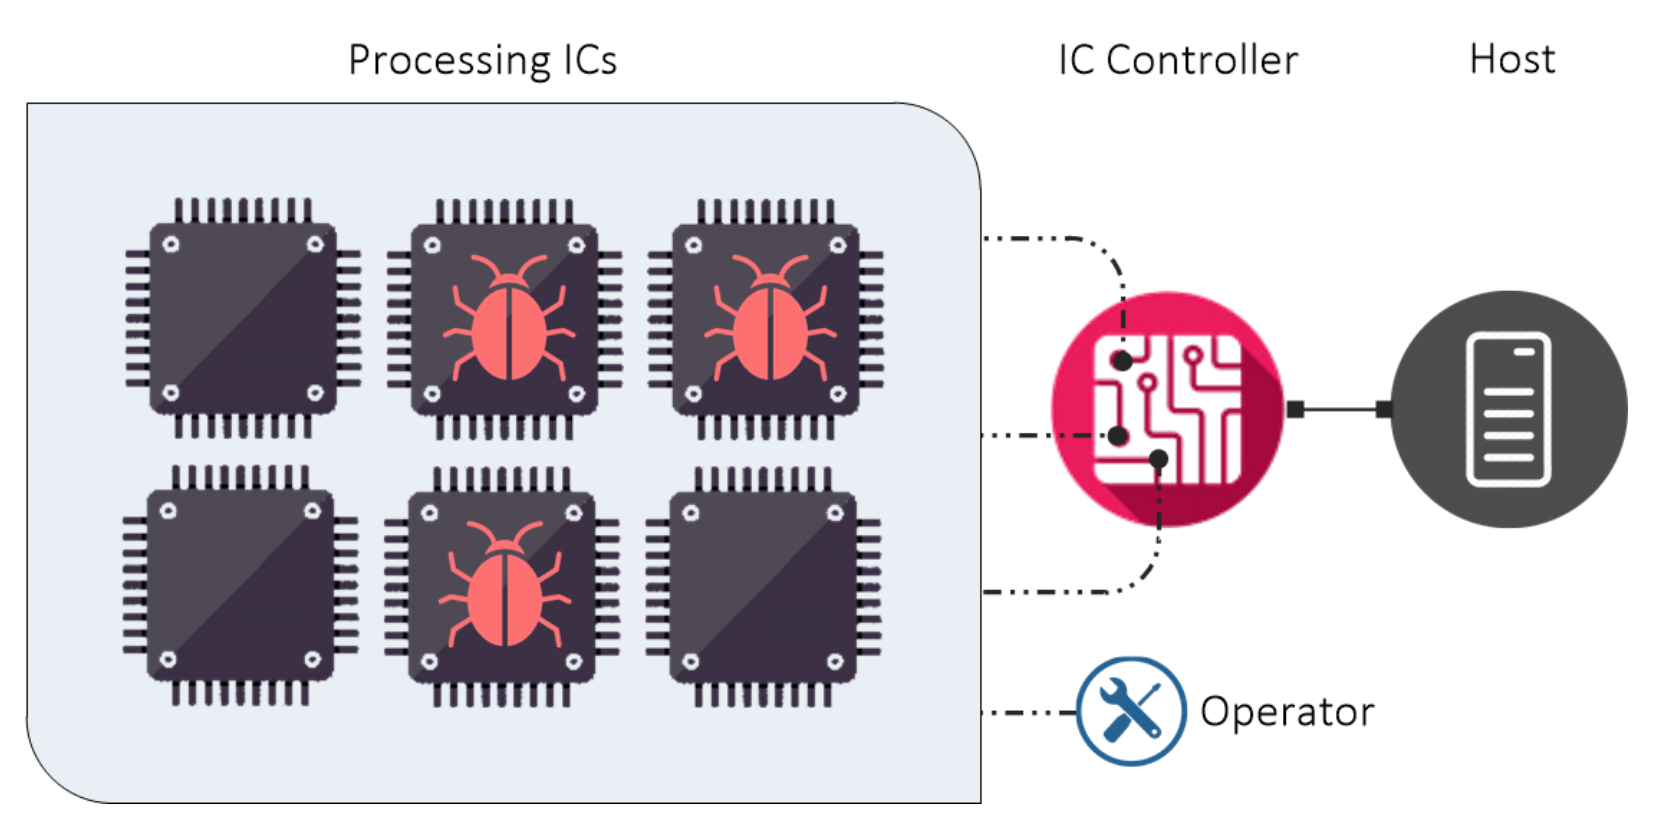
\includegraphics[scale=0.30,clip]{img/myst_arch.png}}%
	{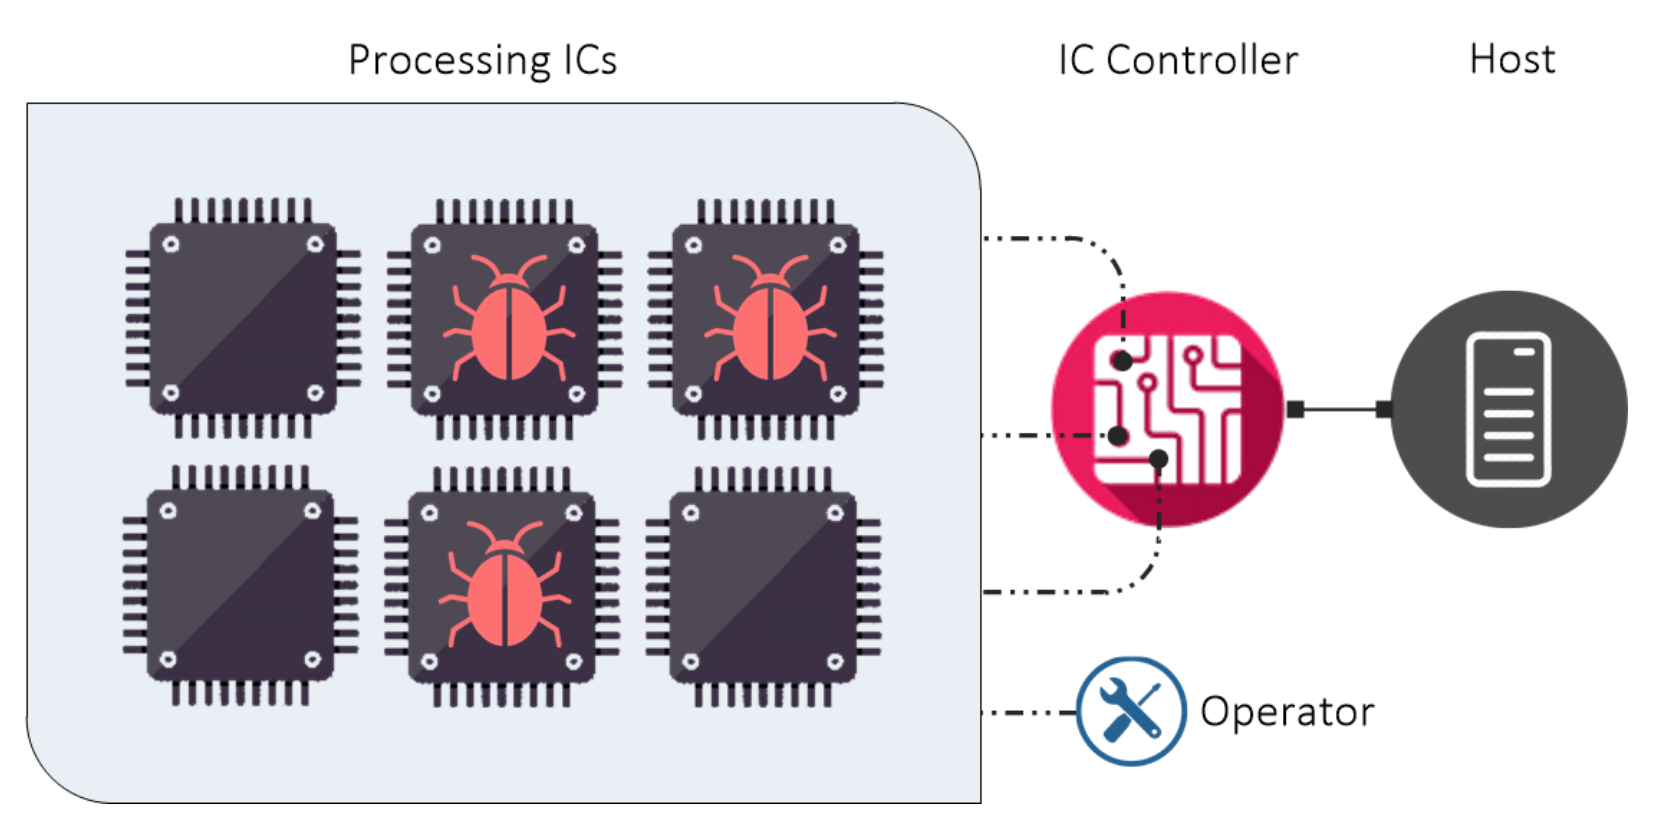
\includegraphics[scale=0.30,clip]{img/myst_arch.png}}
	\captionsetup{width=0.95\linewidth}
	\caption{Architecture of the \emph{Myst}, scalable MPC system designed in \cite{2017-ccs-mavroudis}. IC stands for integrated circuits, which are instantiated by smartcards in our work.}
	\label{fig:myst_arch}
\end{figure}

The distributed key generation operation enables multiple cards to
collectively generate a shared public and private key pair with
shares distributed between all participating cards. The individual card does not have an access to the generated key and the protocol protects from maliciously crafted shares. ElGamal \cite{Brandt:2005:ECP:2182226.2182233} is used for distributed encryption and decryption using the previously generated key shares. For the distributed signing, we introduced a new multi-signature protocol based on Schnorr signatures \cite{Schnorr:1991:ESG:2724954.2725006}.

Myst is a practical solution protecting from single-point-of-failure problems on smartcards. The testing prototype contains 120 individual smartcards with high encryption, decryption and signing throughput as showed in figure \ref{fig:myst_throughput}. Myst is a scalable replacement for Hardware Security Modules (HSM) as the used cards are FIPS 140-2 Level 4 tamper-resistance certified and thanks to our distributed protocols it overcomes potential problems with cryptographic HSM black-box implementation.

\begin{figure}[h]
	\centering
	\ifcamready%
	{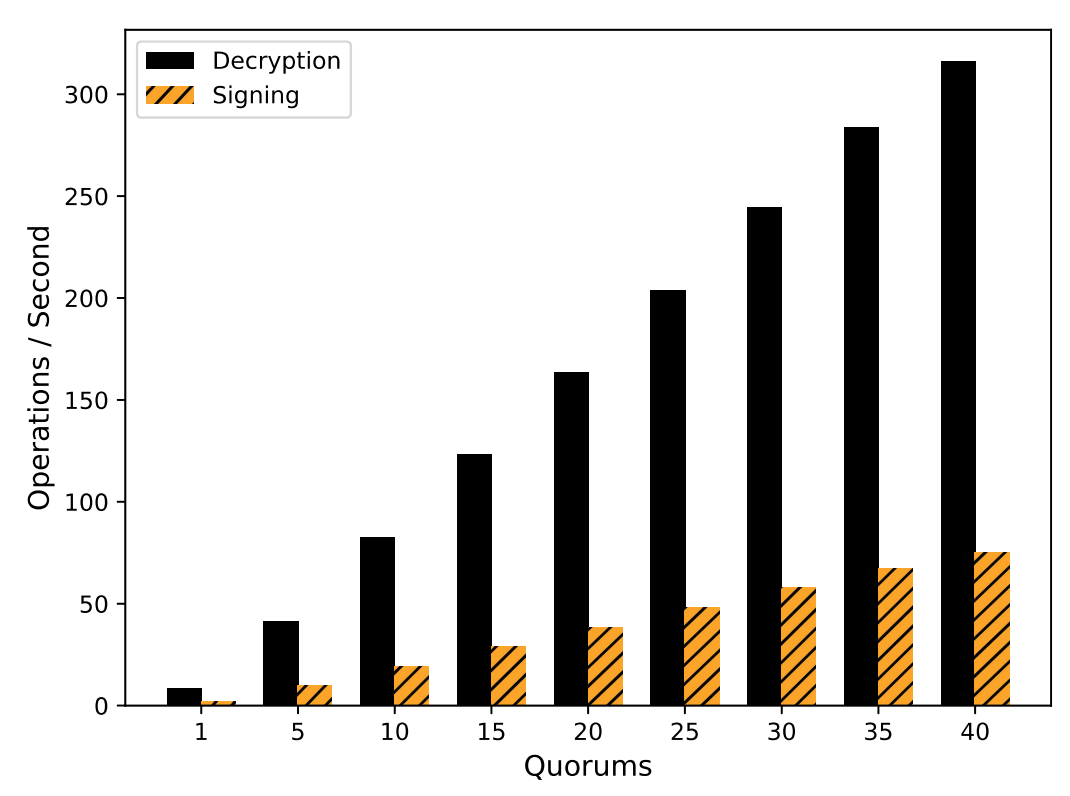
\includegraphics[scale=0.45,clip]{img/myst_throughput.png}}%
	{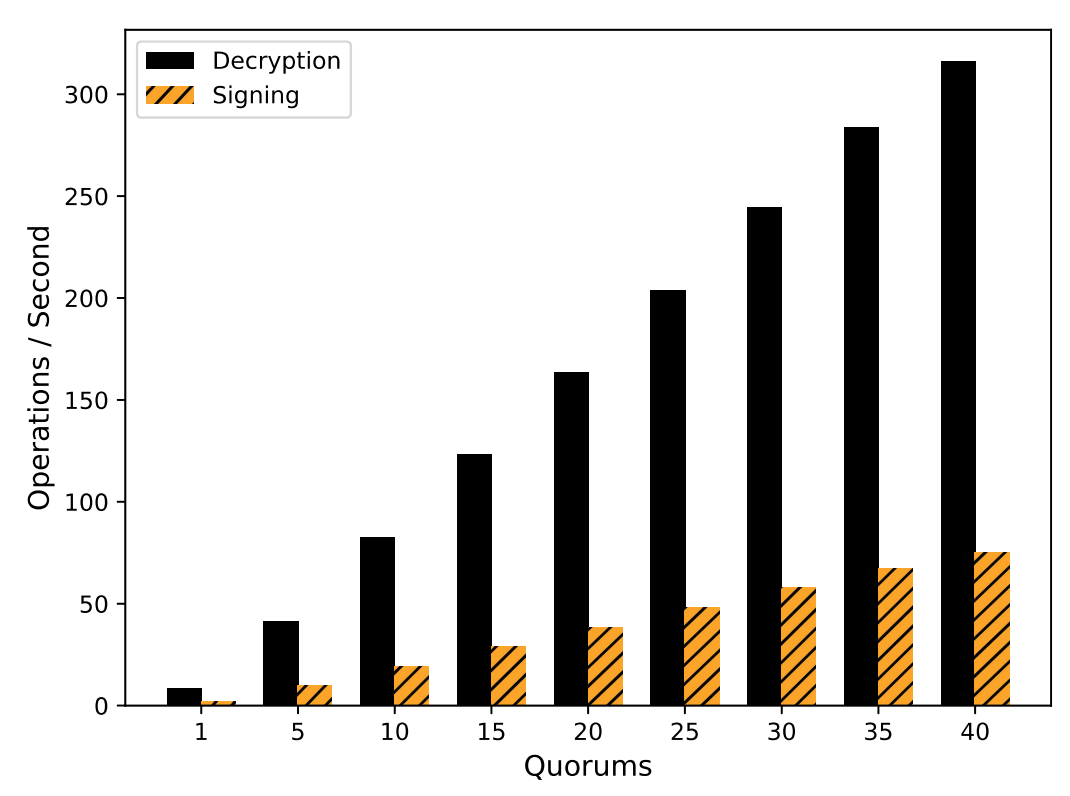
\includegraphics[scale=0.45,clip]{img/myst_throughput.png}}
	\captionsetup{width=0.95\linewidth}
	\caption{Myst average throughput for decryption and signing, depending on the quorum size, i.e., number of cards computing the same operation. From \cite{2017-ccs-mavroudis}.}
	\label{fig:myst_throughput}
\end{figure}

\cite{2017-ccs-mavroudis} was presented on ACM Conference on Computer and Communications Security 2017 (ACM CCS), Dallas, Texas, US.

\section{Monero hardware wallet}
\label{sec:aim:monero_hw_wallet}
In this, yet unpublished, work I designed and implemented transaction signing protocol for Monero~\cite{zero_to_monero}, privacy-centric cryptocurrency, on the hardware wallet, resource constrained device. 

Monero differs from traditional cryptocurrencies in a way it stores the transaction on the blockchain. Transaction sender and recipient are concealed so potential financial flow tracking between participants is severely limited. It uses unique, pseudo-random sender addresses, derived from Diffie-Hellman exchange of the sender and recipient. On top of that, Monero uses ring-signatures to make transaction graph analysis difficult. Ring-signatures are digital signatures which have a \emph{ring} of $N$ public keys associated with it. The signature is verifiable with the whole ring but it is not known which private key corresponding to one public key from the ring actually signed the transaction. This scheme thus provides 1-in-$N$ anonymity.

Monero uses Pedersen commitments to conceal the value of transactions being sent. On top of that, non-interactive zero-knowledge proofs, so-called Bulletproofs \cite{Bnz2017BulletproofsSP} are used to ensure the transaction uses proper values.

In the considered scenario, a user owns a hardware wallet, dedicated device storing the private keys used for signing the transactions. It has usually a display and hardware buttons so user can confirm the transaction details on the device. Hardware wallet protects a user from theft as the key is never leaked to the connected host, which might be infected due to large attack surface and due to its multi-purpose nature. Hardware wallet is on the other hand very limited device so the attack surface is as low as possible. 

I have designed and implemented a Monero transaction signing protocol on a hardware wallet in a way the secret key never leaves the hardware device and the malicious host cannot tamper with the signing data, i.e., user always has to confirm the transaction details first. On top of that, host verifies if the hardware wallet is not cheating either. The protocol is intuitive and it is simple to verify that it preserves desired security properties. It is thus specialized secure two-party computation protocol. 

Later, we plan to extend the protocol to support threshold signatures and multiple different hardware wallets, following the MPC approach of True2F~\cite{DCMBR18} and 
\cite{2017-ccs-mavroudis}. The implementation is already merged to the Monero upstream\footnote{\url{https://github.com/monero-project/monero}} and the Trezor hardware wallet upstream repositories\footnote{\url{https://github.com/trezor/trezor-core/}}.

The paper is not yet published, with expected submission in Spring 2019. 
Preliminary technical report is available on GitHub\footnote{\url{https://github.com/ph4r05/monero-trezor-doc}} and Overleaf\footnote{\url{https://www.overleaf.com/read/bjxshqkrngcy}} \cite{trezor_monero_tech}.
% bulletproofs

\begin{ecmmnt}\subsection{Monero paper}

Idea: submit to Oakland (rolling deadline) or some other A, A+ conference before theses submission. 

Covering basic Monero transaction, transaction signing protocol for hardware wallets, with security proof (ideally. reduction. original signing algorithm is secure then transformed protocol is secure as well).

Covering also blockchain scanning, so view key is not leaked to the host. Schemes designed with their properties. Group payment identification pseudonymity, fast scanning. Encrypted Bloom filters. Impossibility on some attractive scheme properties (publicly derivable public key chain for forward secrecy, corresponding private key derivation only with hardware wallet. Formalize). 
\end{ecmmnt}

\begin{ecmmnt}% summary, my works.
\begin{itemize}
	\item Bug resilience, Kleptography, Single point of failure of resource constrained devices. GACR proposal motivation. eID system failure due to {\bf{ROCA}}~\cite{2017-ccs-nemec}. Smart-ID~\cite{smart_id_ee}. 
	
	- TODO: ROCA 2 paper.
	
	\item {\bf{Fingerprinting}} public keys from cryptographic libraries and devices possible. Enables to target attack on particular vulnerable library. {\bf{ROCA}} also fingerprintable, like shown in our previous research {\it{Measuring Popularity of Cryptographic Libraries in Internet-Wide Scans}}~\cite{2017-acsac-nemec}.
	
	\item In previous research we devised powerful randomness test {\bf{\emph{Booltest}}} \cite{booltest_secrypt2017} which provides comparable and better results compared to standard randomness testing batteries. Testing randomness of PRNGs or cryptographic primitives is essential for the assessment of the quality of cryptographic schemes. It is usually the first step of a security audit. In the extended version of the paper submitted to the Springer Book of Secrypt We also tested output of TRNGs of smartcards and hardware wallets Trezor and Ledger. Having device failing to pass randomness test indicates a further problem with potentially high impact. Implementing the SMPC may help to avoid similar vulnerabilities and potential backdoors. 
	
	\item Many scenarios (e.g., DRM, licensing, cloud assisted computation) require computation with sensitive data on attacker computer. Universal approach is FHE but not practical. Another solution is a secure multi-party computation (SMPC), utilizing secure crypto processors (SCPs) or smartcards to provide better security guarantees. {\bf{Whitebox}} attack resistant cryptography \cite{whitebox_klinec_santacrypt2013,Klinec2013thesis} attempts to transform algorithms so their evaluation on attackers computer is secure, e.g. AES algorithm with embedded decryption key without possibility of key extraction. However, whitebox schemes often fail (cite) which indicates SMPC / SCP schemes are more practical.
	
	\item In previous research, we proposed and analyzed an Intrusion detection system running on resource-constrained devices creating wireless sensor networks \cite{wsnprotectlayer}. Effective multi-party computation algorithms could improve security properties of {\bf{WSN}} protocols.
	
	\item SMPC with Smartcards as our previous research A {\it {\bf{Touch of Evil}}: High-Assurance Cryptographic Hardware from Untrusted Components} \cite{2017-ccs-mavroudis}. Multi-Encryption and multi-signatures N-of-N. At least one honest participant is enough to protect secret.
	
	\item Paper with V. Sedlacek analyzing particular {\bf{number factorization}} method based on elliptic curves. Submitted by the end of theses submission deadline.
	
\end{itemize}
\end{ecmmnt}

\section{Publications}

%\newcommand{\citemypub}[1]{\citetitle{#1} \cite{#1}. }
\newcommand{\citemypub}[1]{\cite{#1}: \fullcite{#1}.\newline}

\begin{itemize}
	%\item \emph{A Touch of Evil: High-Assurance Cryptographic Hardware from Untrusted Components \cite{2017-ccs-mavroudis}.} %
	\item \citemypub{2017-ccs-mavroudis}
	I helped with implementation of the back-end related services for controlling the Myst from the host. Contribution: 5\%
	
	%\item \emph{The Return of Coppersmith's Attack: Practical Factorization of Widely Used RSA Moduli \cite{2017-ccs-nemec}.} %
	\item \citemypub{2017-ccs-nemec}
	I reviewed the math code, implemented the fingerprinting tool\footnote{\url{https://github.com/crocs-muni/roca}}, analyzed large key datasets for presence of the vulnerability, e.g., TLS datasets, certificate authority (CA) keys and Estonian eID. Contribution: 10\%. \todo{DUNNO. CHECK}
	
	%\item \emph{The Efficient Randomness Testing using Boolean Functions \cite{booltest_secrypt2017}}. %
	\item \citemypub{booltest_secrypt2017}
	I co-authored and implemented the Booltest, a tool\footnote{\url{https://github.com/ph4r05/polynomial-distinguishers}} for effective randomness testing. Contribution: 20\%.\todo{DUNNO. CHECK}
	
	%\item \emph{Measuring Popularity of Cryptographic Libraries in Internet-Wide Scans \cite{2017-acsac-nemec}}. %
	\item \citemypub{booltest_secrypt2017}
	I've co-analyzed large key datasets for known fingerprints. Contribution: 20\%.\todo{DUNNO. CHECK}
	
	%\item \emph{Traversing Symmetric NAT with Predictable Port Allocation \cite{Klinec:2014:TSN:2659651.2659698}}. %
	\item \citemypub{Klinec:2014:TSN:2659651.2659698}
	I have designed, implemented and evaluated a protocol for bypassing Symmetric NAT so two parties can establish a direct connection. Contribution: 80\%.
	
	%\item \emph{Android APK on-the-fly tampering \cite{apk_tampering}}. %
	\item \citemypub{apk_tampering}
	I've helped with the design and implementation of the malicious traffic interceptor adding malicious payload to the Android application archives (APKs) being downloaded on-the-fly. Contribution: 40\%.\todo{DUNNO. CHECK}
	
	%\item \emph{WSNProtectLayer – security middleware for wireless sensor networks \cite{wsnprotectlayer}}. %
	\item \citemypub{wsnprotectlayer}
	I co-authored the implementation of the WSNProtectLayer on resource-constrained devices (sensor nodes). Contribution: 5\%.\todo{DUNNO. CHECK}
\end{itemize}

Moreover, there are several papers in the pipeline which have not yet been submitted and are to be finalized in the upcoming months:

\begin{itemize}
	\item \emph{Monero hardware wallet signing protocol.} As mentioned in the Section \ref{sec:aim:monero_hw_wallet}, I have designed and implemented distributed transaction signing protocol. Contribution: 80\%.
	
	\item \emph{The $4p-1$ factorization method and its viability as a basis for an RSA backdoor}. The work describes very effective factorization methods for RSA moduli assuming the private keys are of a special form. I have performed the large-scale algorithm testing and running time analysis. Contribution: 13\%.\todo{DUNNO. CHECK}
	
	\item \emph{Security margins for known cryptographic algorithms.} The work analyzes the security margins of known round-reduced block and stream encryption algorithms and hash functions. I have tested the algorithms with the BoolTest. Contribution: 10\%.\todo{DUNNO. CHECK}	
\end{itemize}

%\section{Papers in progress}
%\begin{itemize}
%	\item ROCA - extended attack. Returning information to the system.
%	
%	\item Automated Smartcard APDU AFL assisted fuzzer with systematic power trace analysis feedback.
%	
%	\item Zero knowledge proof of secrets generation correctness for smartcards. Producing a proof that given public key was generated according to the prescribed standard and thus cannot contain a bug / kleptography backdoor. 
%	
%	\item Static Rabin-Miller basis on embedded cards, testing, detection, exploitation. Based on Bleichenbacher \cite{10.1007/978-3-540-30580-4_2}.
%\end{itemize}


\newpage
\begin{shaded}
\begin{itemize}
    \item What we have, created
    \item Conferences presented
    \item Range: 3-5 pages
\end{itemize}
\end{shaded}

\newpage

%%%%%%%%%%%%%%%%%%%%%%%%%%%%%%%%%%%%%%%%%%%%%%%%%%%%%%%%%%%%%%%%%%%%%%%%%%%%%%%%%%%%%%%%%%%

%\chapter{Author's Publications}
%\begin{shaded}
%\begin{itemize}
%    \item Contribution to the paper, percentual contribution
%\end{itemize}
%\end{shaded}
%
%\todoin{Publications here}


%%%%%%%%%%%%%%%%%%%%%%%%%%%%%%%%%%%%%%%%%%%%%%%%%%%%%%%%%%%%%%%%%%%%%%%%%%%%%%%%%%%%%%%%%%%

%% Bibliography
  \printbibliography[heading=bibintoc] 


%% Index
%   \makeatletter\thesis@blocks@clear\makeatother
%   \phantomsection %% Print the index and insert it into the
%   \addcontentsline{toc}{chapter}{\indexname} %% table of contents.
%   \printindex


%% Appendix
\appendix 

\chapter{Attached papers}
\todoin{Attach papers}

\begin{ecmmnt} % paper list
\section{Monero paper}
Submitted (ideally). Main author, 70\%.

\section{A Touch of Evil: High-Assurance Cryptographic Hardware from Untrusted Components}
Primarily targeting topic, 5\% \cite{2017-ccs-mavroudis}

\section{The Return of Coppersmith's Attack: Practical Factorization of Widely Used RSA Moduli}
ROCA. Motivation for SMPC, 5-10\% \cite{2017-ccs-nemec}.
Add ROCA extension.

\section{The Efficient Randomness Testing using Boolean Functions}
Booltest. \cite{booltest_secrypt2017}.
Add Booltest extended paper in journal.

\section{Measuring Popularity of Cryptographic Libraries in Internet-Wide Scans}
Fingerprinting. Significant contribution 20-30 \% \cite{2017-acsac-nemec}

\section{WSNProtectLayer – security middleware for wireless sensor networks}
Minor contribution. Resource-restricted devices. \cite{wsnprotectlayer}

\section{Whitebox attack resistant cryptography}
\cite{whitebox_klinec_santacrypt2013, Klinec2013thesis} 

- Citations count 9: \url{https://scholar.google.com/scholar?cites=3284880228025768764&as_sdt=2005&sciodt=0,5&hl=sk}

\section{Nat traversal}
\cite{Klinec:2014:TSN:2659651.2659698},
\emph{Traversing Symmetric NAT with Predictable Port Allocation} in the context of establishing P2P connections so parties can communicate directly, e.g., for MPC.


\section{ECC Factorization paper}
Submitted, V. Sedlacek, small contribution, running experiments, results aggregation. 

\section{Papers in progress}
\begin{itemize}
	\item ROCA - extended attack. Returning information to the system.
    
	\item Automated Smartcard APDU AFL assisted fuzzer with systematic power trace analysis feedback.
    
    \item Zero knowledge proof of secrets generation correctness for smartcards. Producing a proof that given public key was generated according to the prescribed standard and thus cannot contain a bug / kleptography backdoor. 
    
    \item Static Rabin-Miller basis on embedded cards, testing, detection, exploitation. Based on Bleichenbacher \cite{10.1007/978-3-540-30580-4_2}.
    
\end{itemize}
\end{ecmmnt}

\chapter{Security models}
\label{apx:uc}
Here we shortly compare plain and security UC model.

\paragraph{Plain model.}
Both models, plain and UC, define two separate worlds.
The \emph{ideal world}, where the security is intuitively guaranteed and the \emph{real world}.

In the ideal world, the \emph{ideal~functionality}\footnote{Ideal functionality was originally used in~\cite{GMW87}.} $\mathcal{F}$ is a natural algorithmic description of the function $f$. It securely evaluates the function $f$ acting as an incorruptible trusted third party (TTP). It securely evaluates $f$ and returns the result to the participants $P_i$. The \emph{adversary}~$\mathcal{A}$ can interact with $\mathcal{F}$ only via the external interface. Besides that, $\mathcal{A}$ interacts with other parties in an arbitrary manner, defined by the security properties being proved, e.g. semi-honest vs. malicious adversary.
This notion intuitively captures the desired security properties we want the protocol $\pi$ realizing function $f$ to have, i.e., it should securely emulate the TTP in the real world setting.

We say that $\pi$ securely evaluates a function $f$ in the real world if for any adversary $\mathcal{A}$ there exists an ideal adversary $\mathcal{S}$, a simulator, such that statistical distributions generated by views of parties in the real world and ideal world are indistinguishable. 

\begin{definition}
	We call a function $\mu$ : $\mathbb{N} \leftarrow [0,1]$ \emph{negligible} in $x$ if for all $c \in \mathbb{N}$ there exists $x_c \in \mathbb{N}$ such that $\mu(x) \leq x^{-c}$ for all $x > x_c$.
\end{definition}

If all non-uniform polynomial time distinguisher can distinguish the distributions only with negligible probability the security is \emph{computational}. If the statistical distance of distributions is negligible then the protocol is \emph{statistically secure}, without computational restrictions on the distinguishers.
If the distributions are perfectly equal we say the security is \emph{perfect}. 

%The \emph{view} of a party is defined contains the input, internal randomness and all received messages during the protocol.

\paragraph{UC framework.}
The UC framework captures a complex set of interactions in comparison to the plain-model. MPC protocols may be executed with the same or other parties, parties inputs may be correlated, protocol outputs can be used by other protocols and message communication could be controlled by an adversary in any way. 

It is not feasible to address all these concerns in the plain model as one would have to model each individually. Still, there would be new, previously neglected problems. These concerns motivated quick shift to UC framework which provides very high-security guarantees.

The power stems from the addition of an \emph{environment}~$\mathcal{Z}$, the algorithmic entity that represents everything external to the protocol execution, representing potential outside interactions and concurrent protocol executions. It wraps and controls the execution, hands arbitrary inputs to the parties, collects outputs from the parties, communicates with the adversary~$\mathcal{A}$ during the whole course of the protocol. The communication with~$\mathcal{A}$ is essential to the security.

%This notion intuitively captures the desired security properties we want the protocol $\pi$ realizing function $f$ to have, i.e., it should securely emulate the TTP in the real world setting.

We say that $\pi$ securely evaluates a function $f$ if for any adversary $\mathcal{A}$ there exists an ideal adversary $\mathcal{S}$, a simulator, such that no environment $\mathcal{Z}$ can with non-negligible advantage distinguish the real-world ($\pi, \mathcal{A}$) and the ideal world ($\mathcal{F}, \mathcal{S}$). The environment $\mathcal{Z}$ is running in the time \emph{similar} to the adversary, i.e., polynomially to $\mathcal{A}$.

If not said otherwise, the adversary is considered to be running in probabilistic polynomial-time (computational security). In the model with private communication channels, it makes sense to assume also computationally unbounded adversaries. Then like in the plain model we talk about \emph{statistical} and \emph{perfect} security.

For more detailed treatment please refer to \cite{Can01, CLOS02, Lin03, G09, CDN15, Lin17}.

\end{document}


%%%%%%%%%%%%%%%%%%%%%%%%%%%%%%%%%%%%%%%%%%%%%%%%%%%%%%%%%%%%%%%%%%%%%%%%
%% Trash
%%%%%%%%%%%%%%%%%%%%%%%%%%%%%%%%%%%%%%%%%%%%%%%%%%%%%%%%%%%%%%%%%%%%%%%%


%Theses are rumoured to be the capstones of education, so I decided
%to write one of my own. If all goes well, I will soon have a
%diploma under my belt. Wish me luck!


%\begin{otherlanguage}{czech}
%czz
%\end{otherlanguage}

%\chapter{These are}
%\section{the available}
%\subsection{sectioning}
%\subsubsection{commands.}
%\paragraph{Paragraphs and}
%\subparagraph{subparagraphs are available as well.}
%Inside the text, you can also use unnumbered lists,
%\begin{itemize}
%  \item such as
%   \item this one
%   \begin{itemize}
%     \item     and they can be nested as well.
%     \item[>>] You can even turn the bullets into something fancier,
%     \item[\S] if you so desire.
%   \end{itemize}
% \end{itemize}
% Numbered lists are
% \begin{enumerate}
%   \item very
%   \begin{enumerate}
%     \item similar
%   \end{enumerate}
% \end{enumerate}
% and so are description lists:
% \begin{description}
%   \item[Description list]
%     A list of terms with a description of each term
% \end{description}
% The spacing of these lists is geared towards paragraphs of text.
% For lists of words and phrases, the \textsf{paralist} package
% offers commands
% \begin{compactitem}
%   \item that
%   \begin{compactitem}
%     \item are
%     \begin{compactitem}
%       \item better
%       \begin{compactitem}
%         \item suited
%       \end{compactitem}
%     \end{compactitem}
%   \end{compactitem}
% \end{compactitem}
% \begin{compactenum}
%   \item to
%   \begin{compactenum}
%     \item this
%     \begin{compactenum}
%       \item kind of
%       \begin{compactenum}
%         \item content.
%       \end{compactenum}
%     \end{compactenum}
%   \end{compactenum}
% \end{compactenum}
% The \textsf{amsthm} package provides the commands necessary for the
% typesetting of mathematical definitions, theorems, lemmas and
% proofs.

%% We will define several mathematical sectioning commands.
%\newtheorem{theorem}{Theorem}[section] %% The numbering of theorems
%                               %% will be reset after each section.
%\newtheorem{lemma}[theorem]{Lemma}         %% The numbering of lemmas
%\newtheorem{corollary}[theorem]{Corollary} %% and corollaries will
%                               %% share the counter with theorems.
%\theoremstyle{definition}
%\newtheorem{definition}{Definition}
%\theoremstyle{remark}
%\newtheorem*{remark}{Remark}

% \begin{theorem}
%   This is a theorem that offers a profound insight into the
%   mathematical sectioning commands.
% \end{theorem}
% \begin{theorem}[Another theorem]
%   This is another theorem. Unlike the first one, this theorem has
%   been endowed with a name.
% \end{theorem}
% \begin{lemma}
%   Let us suppose that $x^2+y^2=z^2$. Then
%   \begin{equation}
%     \biggl\langle u\biggm|\sum_{i=1}^nF(e_i,v)e_i\biggr\rangle
%     =F\biggl(\sum_{i=1}^n\langle e_i|u\rangle e_i,v\biggr).
%   \end{equation}
% \end{lemma}
% \begin{proof}
%   $\nabla^2 f(x,y)=\frac{\partial^2f}{\partial x^2}+
%    \frac{\partial^2f}{\partial y^2}$.
% \end{proof}
% \begin{corollary}
%   This is a corollary.
% \end{corollary}
% \begin{remark}
%   This is a remark.
% \end{remark}

% \chapter{Floats and references}
% \begin{figure}
%   \begin{center}
%     %% PNG and JPG images can be inserted into the document as well,
%     %% but their resolution needs to be adequate. The minimum is
%     %% about 100 pixels per 1 centimeter or 300 pixels per 1 inch.
%     %% That means that a JPG or PNG image typeset at 4 × 4 cm should
%     %% be 400 × 400 px large at the bare minimum.
%     %%
%     %% The optimum is about 250 pixels per 1 centimeter or 600
%     %% pixels per 1 inch. That means that a JPG or PNG image typeset
%     %% at 4 × 4 cm should be 1000 × 1000 px large or larger.
%     
\includegraphics[width=4cm]{fithesis/logo/mu/fithesis-base.pdf}
%   \end{center}
%   \caption{The logo of the Masaryk University at 40\,mm}
%   \label{fig:mulogo1}
% \end{figure}

% \begin{figure}
%   \begin{center}
%     \begin{minipage}{.66\textwidth}
%       
\includegraphics[width=\textwidth]{fithesis/logo/mu/fithesis-base.pdf}
%     \end{minipage}
%     \begin{minipage}{.33\textwidth}
%       
\includegraphics[width=\textwidth]{fithesis/logo/mu/fithesis-base.pdf} \\
%       
\includegraphics[width=\textwidth]{fithesis/logo/mu/fithesis-base.pdf}
%     \end{minipage}
%   \end{center}
%   \caption{The logo of the Masaryk University at $\frac23$ and
%     $\frac13$ of text width}
%   \label{fig:mulogo2}
% \end{figure}

% \begin{table}
%   \begin{tabularx}{\textwidth}{lllX}
%     \toprule
%     Day & Min Temp & Max Temp & Summary \\
%     \midrule
%     Monday & $13^{\circ}\mathrm{C}$ & $21^\circ\mathrm{C}$ & A
%     clear day with low wind and no adverse current advisories. \\
%     Tuesday & $11^{\circ}\mathrm{C}$ & $17^\circ\mathrm{C}$ & A
%     trough of low pressure will come from the northwest. \\
%     Wednesday & $10^{\circ}\mathrm{C}$ &
%     $21^\circ\mathrm{C}$ & Rain will spread to all parts during the
%     morning. \\
%     \bottomrule
%   \end{tabularx}
%   \caption{A weather forecast}
%   \label{tab:weather}
% \end{table}

% The logo of the Masaryk University is shown in Figure
% \ref{fig:mulogo1} and Figure \ref{fig:mulogo2} at pages
% \pageref{fig:mulogo1} and \pageref{fig:mulogo2}. The weather
% forecast is shown in Table \ref{tab:weather} at page
% \pageref{tab:weather}. The following chapter is Chapter
% \ref{chap:matheq} and starts at page \pageref{chap:matheq}.
% Items \ref{item:star1}, \ref{item:star2}, and
% \ref{item:star3} are starred in the following list:
% \begin{compactenum}
%   \item some text
%   \item some other text
%   \item $\star$ \label{item:star1}
%   \begin{compactenum}
%     \item some text
%     \item $\star$ \label{item:star2}
%     \item some other text
%     \begin{compactenum}
%       \item some text
%       \item some other text
%       \item yet another piece of text
%       \item $\star$ \label{item:star3}
%     \end{compactenum}
%     \item yet another piece of text
%   \end{compactenum}
%   \item yet another piece of text
% \end{compactenum}
% If your reference points to a place that has not yet been typeset,
% the \verb"\ref" command will expand to \textbf{??} during the first
% run of
% \texttt{pdflatex \jobname.tex}
% and a second run is going to be needed for the references to
% resolve. With online services -- such as Overleaf -- this is
% performed automatically.

% \chapter{Mathematical equations}
% \label{chap:matheq}
% \TeX{} comes pre-packed with the ability to typeset inline
% equations, such as $\mathrm{e}^{ix}=\cos x+i\sin x$, and display
% equations, such as \[
%   \mathbf{A}^{-1} = \begin{bmatrix}
%   a & b \\ c & d \\
%   \end{bmatrix}^{-1} =
%   \frac{1}{\det(\mathbf{A})} \begin{bmatrix}
%   \,\,\,d & \!\!-b \\ -c & \,a \\
%   \end{bmatrix} =
%   \frac{1}{ad - bc} \begin{bmatrix}
%   \,\,\,d & \!\!-b \\ -c & \,a \\
%   \end{bmatrix}.
% \] \LaTeX{} defines the automatically numbered \texttt{equation}
% environment:
% \begin{equation}
%   \gamma Px = PAx = PAP^{-1}Px.
% \end{equation}
% The package \textsf{amsmath} provides several additional
% environments that can be used to typeset complex equations:
% \begin{enumerate}
%   \item An equation can be spread over multiple lines using the
%     \texttt{multline} environment:
%     \begin{multline}
%       a + b + c + d + e + f + b + c + d + e + f + b + c + d + e +
% f \\
%       + f + g + h + i + j + k + l + m + n + o + p + q
%     \end{multline}

%   \item Several aligned equations can be typeset using the
%     \texttt{align} environment:
%     \begin{align}
%               a + b &= c + d     \\
%                   u &= v + w + x \\[1ex]
%       i + j + k + l &= m
%     \end{align}

%   \item The \texttt{alignat} environment is similar to
%     \texttt{align}, but it doesn't insert horizontal spaces between
%     the individual columns:
%     \begin{alignat}{2}
%       a + b + c &+ d       &   &= 0 \\
%               e &+ f + g   &   &= 5
%     \end{alignat}

%   \item Much like chapter, sections, tables, figures, or list
%     items, equations -- such as \eqref{eq:first} and
%     \eqref{eq:mine} -- can also be labeled and referenced:
%     \begin{alignat}{4}
%       b_{11}x_1 &+ b_{12}x_2  &  &+ b_{13}x_3  &  &             &
%         &= y_1,                   \label{eq:first} \\
%       b_{21}x_1 &+ b_{22}x_2  &  &             &  &+ b_{24}x_4  &
%         &= y_2. \tag{My equation} \label{eq:mine}
%     \end{alignat}

%   \item The \texttt{gather} environment makes it possible to
%     typeset several equations without any alignment:
%     \begin{gather}
%       \psi = \psi\psi, \\
%       \eta = \eta\eta\eta\eta\eta\eta, \\
%       \theta = \theta.
%     \end{gather}

%   \item Several cases can be typeset using the \texttt{cases}
%     environment:
%     \begin{equation}
%       |y| = \begin{cases}
%         \phantom-y & \text{if }z\geq0, \\
%                 -y & \text{otherwise}.
%       \end{cases}
%     \end{equation}
% \end{enumerate}
% For the complete list of environments and commands, consult the
% \textsf{amsmath} package manual\footnote{
%   See \url{http://mirrors.ctan.org/macros/latex/required/amslatex/math/amsldoc.pdf}.
%   The \texttt{\textbackslash url} command is provided by the
%   package \textsf{url}.
% }.

% \chapter{\textnormal{We \textsf{have} \texttt{several} \textsc{fonts}
%   \textit{at} \textbf{disposal}}}
% The serified roman font is used for the main body of the text.
% \textit{Italics are typically used to denote emphasis or
% quotations.} \texttt{The teletype font is typically used for source
% code listings.} The \textbf{bold}, \textsc{small-caps} and
% \textsf{sans-serif} variants of the base roman font can be used to
% denote specific types of information.

% \tiny We \scriptsize can \footnotesize also \small change \normalsize
% the \large font \Large size, \LARGE although \huge it \Huge
% is \huge usually \LARGE not \Large necessary.\normalsize

% A wide variety of mathematical fonts is also available, such as: \[
%   \mathrm{ABC}, \mathcal{ABC}, \mathbf{ABC}, \mathsf{ABC},
%   \mathit{ABC}, \mathtt{ABC}
% \] By loading the \textsf{amsfonts} packages, several additional
% fonts will become available: \[
%   \mathfrak{ABC}, \mathbb{ABC}
% \] Many other mathematical fonts are available\footnote{
%   See \url{http://tex.stackexchange.com/a/58124/70941}.
% }.

% \chapter{Using lightweight markup}
% \shorthandoff{-}
% \begin{markdown*}{%
%   hybrid,
%   definitionLists,
%   footnotes,
%   inlineFootnotes,
%   hashEnumerators,
%   fencedCode,
%   citations,
%   citationNbsps,
% }

% If you decide that \LaTeX{} is too wordy for some parts of your
% document, there are [packages](https://www.ctan.org/pkg/markdown
% "Markdown") that allow you to use more lightweight markup next
% to it.

%  ![logo](fithesis/logo/mu/fithesis-base.pdf "The logo of the
%   Masaryk University")

% This is a bullet list. Unlike numbered lists, bulleted lists
% contain an **unordered** set of bullet points. When a bullet point
% contains multiple paragraphs, the list is typeset as follows:

%   * The first item of a bullet list

%     that spans several paragraphs,
%   * the second item of a bullet list,
%   * the third item of a bullet list.

% When none of the bullet points contains multiple paragraphs, the
% list has a more compact form:

%   * The first item of a bullet list,
%   * the second item of a bullet list,
%   * the third item of a bullet list.

% Unlike a bulleted list, a numbered list implies chronology or
% ordering of the bullet points. When a bullet point
% contains multiple paragraphs, the list is typeset as follows:

%   1. The first item of an ordered list

%      that spans several paragraphs,
%   2. the second item of an ordered list,
%   3. the third item of an ordered list.
%   #. If you are feeling lazy,
%   #. you can use hash enumerators as well.

% When none of the bullet points contains multiple paragraphs, the
% list has a more compact form:

%   6. The first item of an ordered list,
%   7. the second item of an ordered list,
%   8. the third item of an ordered list.

% Definition lists are used to provide definitions of terms. When
% a definition contains multiple paragraphs, the list is typeset
% as follows:

% Term 1

% :   Definition 1

% *Term 2*

% :   Definition 2

%         Some code, part of Definition 2

%     Third paragraph of Definition 2.

% When none of the bullet points contains multiple paragraphs, the
% list has a more compact form:

% Term 1
% :   Definition 1
% *Term 2*
% :   Definition 2

% Block quotations are used to include an excerpt from an external
% document in way that visually clearly separates the excerpt from
% the rest of the work:

% > This is the first level of quoting.
% >
% > > This is nested blockquote.
% >
% > Back to the first level.

% Footnotes are used to include additional information to the
% document that are not necessary for the understanding of the main
% text. Here is a footnote reference^[Here is the footnote.] and
% another.[^longnote]

% [^longnote]: Here's one with multiple blocks.

%     Subsequent paragraphs are indented to show that they
% belong to the previous footnote.

%         Some code

%     The whole paragraph can be indented, or just the first
%     line.  In this way, multi-paragraph footnotes work like
%     multi-paragraph list items.

% Citations are used to provide bibliographical references to other
% documents. This is a regular citation~[@borgman03, p. 123]. This is
% an in-text citation: @borgman03\. You can also cite several authors
% at once using both regular~[see @borgman03, p. 123; @greenberg98,
% sec.  3.2; and @thanh01] and in-text citations: @borgman03 [p.123;
% @greenberg98, sec. 3.2; @thanh01].

% Code blocks are used to include source code listings into the
% document:

%     #include <stdio.h>
%     #include <unistd.h>
%     #include <sys/types.h>
%     #include <sys/wait.h>
%     // This is a comment
%     int main(int argc, char **argv)
%     {
%         while (--c > 1 && !fork());
%         sleep(c = atoi(v[c]));
%         printf("%d\n", c);
%         wait(0);
%         return 0;
%     }

% There is an alternative syntax for code blocks that allows you to
% specify additional information, such as the language of the source
% code. This information can be used for syntax highlighting:

% ``` sh
% #!/bin/sh
% fac() {
%   if [ "$1" -leq 1 ]; then
%     echo 1
%   else
%     echo $(("$1" * fac $(("$1" - 1))))
%   fi
% }
% ``````````````

% ~~~~~~ Ruby
% # Here's a way to empty an array.
% joe = [ 'eggs.', 'some', 'break', 'to', 'Have' ]
% print(joe.pop, " ") while joe.size > 0
% print "\n"
% ~~~~~~

% \end{markdown*}
% \shorthandon{-}

% \chapter{Inserting the bibliography}
% After linking a bibliography data\-base files to the document using
% the \verb"\"\texttt{thesis\discretionary{-}{}{}setup\{bib\discretionary{=}{=}{=}

% \{\textit{file1},\textit{file2},\,\ldots\,\}\}} command, you can
% start citing the entries. This is just dummy text
% \parencite{borgman03} lightly sprinkled with citations
% \parencite[p.~123]{greenberg98}. Several sources can be cited at
% once: \cite{borgman03,greenberg98,thanh01}.
% \citetitle{greenberg98} was written by \citeauthor{greenberg98} in
% \citeyear{greenberg98}. We can also produce \textcite{greenberg98}%
% \ or %% Let us define a compound command:
% \def\citeauthoryear#1{(\textcite{#1},~\citeyear{#1})}%
% \citeauthoryear{greenberg98}%
% . The full bibliographic citation is:
% \emph{\fullcite{greenberg98}}. We can easily insert a bibliographic
% citation into the footnote\footfullcite{greenberg98}.

% The \verb"\nocite" command will not generate any
% output\nocite{muni}, but it will insert its arguments into
% the bibliography. The \verb"\nocite{*}" command will insert all the
% records in the bibliography database file into the bibliography.
% Try uncommenting the command
% %% \nocite{*}
% and watch the bibliography section come apart at the seams.

% When typesetting the document for the first time, citing a
% \texttt{work} will expand to [\textbf{work}] and the
% \verb"\printbibliography" command will produce no output. It is now
% necessary to generate the bibliography by running \texttt{biber
% \jobname.bcf} from the command line and then by typesetting the
% document again twice. During the first run, the bibliography
% section and the citations will be typeset, and in the second run,
% the bibliography section will appear in the table of contents.

% The \texttt{biber} command needs to be executed from within the
% directory, where the \LaTeX\ source file is located. In Windows,
% the command line can be opened in a directory by holding down the
% \textsf{Shift} key and by clicking the right mouse button while
% hovering the cursor over a directory.  Select the \textsf{Open
% Command Window Here} option in the context menu that opens shortly
% afterwards.

% With online services -- such as Overleaf -- or when using an
% automatic tool -- such as \LaTeX MK -- all commands are executed
% automatically. When you omit the \verb"\printbibliography" command,
% its location will be decided by the template.


% \chapter{Inserting the index}
% After using the \verb"\makeindex" macro and loading the
% \texttt{makeidx} package that provides additional indexing
% commands, index entries can be created by issuing the \verb"\index"
% command. \index{dummy text|(}It is possible to create ranged index
% entries, which will encompass a span of text.\index{dummy text|)}
% To insert complex typographic material -- such as $\alpha$
% \index{alpha@$\alpha$} or \TeX{} \index{TeX@\TeX} --
% into the index, you need to specify a text string, which will
% determine how the entry will be sorted. It is also possible to
% create hierarchal entries. \index{vehicles!trucks}
% \index{vehicles!speed cars}

% After typesetting the document, it is necessary to generate the
% index by running
% \begin{center}%
%   \texttt{texindy -I latex -C utf8 -L }$\langle$\textit{locale}%
%   $\rangle$\texttt{ \jobname.idx}
% \end{center}
% from the command line, where $\langle$\textit{locale}$\rangle$
% corresponds to the main locale of your thesis -- such as
% \texttt{english}, and then typesetting the document again.

% The \texttt{texindy} command needs to be executed from within the
% directory, where the \LaTeX\ source file is located. In Windows,
% the command line can be opened in a directory by holding down the
% \textsf{Shift} key and by clicking the right mouse button while
% hovering the cursor over a directory. Select the \textsf{Open Command
% Window Here} option in the context menu that opens shortly
% afterwards.

% With online services -- such as Overleaf -- the commands are
% executed automatically, although the locale may be erroneously
% detected, or the \texttt{makeindex} tool (which is only able to
% sort entries that contain digits and letters of the English
% alphabet) may be used instead of \texttt{texindy}. In either case,
% the index will be ill-sorted.


